\documentclass[12pt,a4paper]{article}
\usepackage{iftex}
\ifXeTeX
  \usepackage{fontspec}
  \setmainfont{Times New Roman}
  \setsansfont{Times New Roman}
  \setmonofont{Consolas}
\else
  \usepackage[utf8]{vietnam}
\fi
\usepackage[margin=2cm,top=2.2cm,bottom=2.2cm]{geometry}
\usepackage{amsmath,amssymb}
\usepackage{graphicx}
\usepackage{booktabs}
\usepackage{array}
\usepackage{listings}
\usepackage{xcolor}
\usepackage{tikz}
\usepackage{pgfornament}
\usetikzlibrary{calc}
\usepackage{float}
\usepackage{hyperref}

\hypersetup{
    colorlinks=true,
    linkcolor=black,
    citecolor=black,
    urlcolor=black
}

% Định nghĩa màu sắc cho phần mã nguồn (code listings)
\definecolor{codegreen}{rgb}{0.15,0.55,0.15}
\definecolor{codegray}{rgb}{0.45,0.45,0.45}
\definecolor{codepurple}{rgb}{0.58,0,0.82}
\definecolor{backcolour}{rgb}{0.97,0.97,0.97}
\definecolor{bordercolour}{rgb}{0.85,0.85,0.85}
\definecolor{navyborder}{RGB}{10, 45, 105}

\lstset{
    language=Python,
    backgroundcolor=\color{backcolour},
    commentstyle=\color{codegreen}\itshape,
    keywordstyle=\color{blue}\bfseries,
    numberstyle=\tiny\color{codegray},
    stringstyle=\color{red!70!black},
    basicstyle=\ttfamily\footnotesize,
    breakatwhitespace=false,
    breaklines=true,
    captionpos=b,
    keepspaces=true,
    numbers=left,
    numbersep=7pt,
    showspaces=false,
    showstringspaces=false,
    showtabs=false,
    tabsize=4,
    frame=single,
    rulecolor=\color{bordercolour}
}

\begin{document}
\renewcommand{\contentsname}{\centering\LARGE\textbf{MỤC LỤC}}
\renewcommand{\figurename}{Hình}
\renewcommand{\tablename}{Bảng}

% ==============================================================================
% TRANG BÌA
% ==============================================================================
\begin{titlepage}

\begin{tikzpicture}[remember picture, overlay]
    \draw[line width=1.5pt, color=navyborder] 
        ($(current page.north west) + (1.5cm,-1.5cm)$) 
        rectangle 
        ($(current page.south east) + (-1.5cm,1.5cm)$);
    \draw[line width=0.6pt, color=navyborder] 
        ($(current page.north west) + (1.62cm,-1.62cm)$) 
        rectangle 
        ($(current page.south east) + (-1.62cm,1.62cm)$);
        
    \node[anchor=north west] at ($(current page.north west) + (1.5cm,-1.5cm)$) 
        {\pgfornament[width=1.7cm, color=navyborder]{61}};
    \node[anchor=north east] at ($(current page.north east) + (-1.5cm,-1.5cm)$) 
        {\pgfornament[width=1.7cm, color=navyborder, symmetry=v]{61}};
    \node[anchor=south west] at ($(current page.south west) + (1.5cm,1.5cm)$) 
        {\pgfornament[width=1.7cm, color=navyborder, symmetry=h]{61}};
    \node[anchor=south east] at ($(current page.south east) + (-1.5cm,1.5cm)$) 
        {\pgfornament[width=1.7cm, color=navyborder, symmetry=c]{61}};
\end{tikzpicture}

\centering
\vspace*{0.8cm}

{\textbf{\large TRƯỜNG ĐẠI HỌC CÔNG NGHỆ}\par}
{\textbf{\large ĐẠI HỌC QUỐC GIA HÀ NỘI}\par}

\vspace{1.5cm}


\includegraphics[width=0.46\textwidth]{logo_30_fet.png}

\vspace{1.6cm}

{\textbf{\huge BÁO CÁO THỰC HÀNH BUỔI SÁU}\par}
\vspace{0.4cm}
{\textbf{\LARGE TRÍCH CHỌN ĐẶC TRƯNG ẢNH VÀ ỨNG DỤNG}\par}
\vspace{0.2cm}
{\textbf{\LARGE TRONG CÁC MÔ HÌNH HỌC MÁY}\par}
\vspace{0.2cm}
{\textbf{\Large (KNN, SVM VÀ RANDOM FOREST)}\par}
\vspace{0.4cm}
{\textbf{\large MÔN: XỬ LÝ ẢNH VÀ THỊ GIÁC ROBOT RBE3015}\par}

\vspace{2.2cm}

\begin{flushleft}
\hspace{2.2cm}
\begin{tabular}{ll}
\textbf{Sinh viên thực hiện:} & \textbf{Nguyễn Quang Tuân - 23020767} \\[0.4cm]
\textbf{Giảng viên phụ trách:} & \textbf{PGS.TS. Hoàng Văn Xiêm} \\
                                & \textbf{CN. Bùi Đình Đăng}
\end{tabular}
\end{flushleft}

\vfill
\end{titlepage}

% ==============================================================================
% MỤC LỤC
% ==============================================================================
\newpage
\pagenumbering{roman}
\tableofcontents
\newpage
\pagenumbering{arabic}

% ==============================================================================
% BÀI 1: PHÂN LOẠI ẢNH DỰA TRÊN ĐẶC TRƯNG THỐNG KÊ VÀ MÀU SẮC
% ==============================================================================
\section[BÀI 1: PHÂN LOẠI ẢNH DỰA TRÊN ĐẶC TRƯNG THỐNG KÊ VÀ MÀU SẮC]{BÀI 1: PHÂN LOẠI ẢNH DỰA TRÊN ĐẶC TRƯNG\\THỐNG KÊ VÀ MÀU SẮC}

\subsection{Mục tiêu và yêu cầu đề bài}
\begin{itemize}
    \item \textbf{Mục tiêu:} Trích chọn các đặc trưng thống kê cơ bản từ ảnh số, biểu diễn ảnh bằng vector đặc trưng, xây dựng và đánh giá mô hình KNN và SVM.
    \item \textbf{Dữ liệu đầu vào:} Bộ ảnh ba nhóm đối tượng: táo (\texttt{apple}), chuối (\texttt{banana}) và cam (\texttt{orange}) lấy từ bộ dữ liệu công khai \texttt{Fruits-360} (\texttt{fruits-360-100x100}). Để đảm bảo tính đa dạng về giống quả, góc chụp, độ sáng đồng thời giữ cân bằng lớp, thực nghiệm lấy mẫu phân tầng \textbf{600 ảnh/nhóm} (tổng cộng \textbf{1.800 ảnh}, gấp 12 lần mức tối thiểu 50 ảnh/nhóm của đề bài) trải đều trên toàn bộ 30 thư mục Táo (20 ảnh/thư mục), 6 thư mục Chuối (100 ảnh/thư mục) và 6 thư mục Cam (100 ảnh/thư mục). Ngoài ra trích riêng 12 ảnh hoàn toàn mới từ tập \texttt{Test} để kiểm thử dự đoán nhãn.
    \item \textbf{Các yêu cầu thực hiện:}
    \begin{enumerate}
        \item \textit{Yêu cầu 1 (Tiền xử lý ảnh):} Đọc, hiển thị, thay đổi kích thước ảnh về $128 \times 128$ pixel; chuyển đổi không gian màu từ RGB sang HSV và minh họa kết quả sau các bước.
        \item \textit{Yêu cầu 2 (Trích chọn đặc trưng):} Tính trung bình (Mean) và độ lệch chuẩn (Standard Deviation) cho mỗi kênh màu RGB và HSV; tính Histogram màu HSV và Entropy của ảnh xám; tạo vector đặc trưng cho từng ảnh và trình bày bảng dữ liệu đặc trưng kèm nhãn.
        \item \textit{Yêu cầu 3 (Xây dựng mô hình):} Chia tập dữ liệu Train/Test theo tỷ lệ $80/20$ có phân tầng theo nhãn; chuẩn hóa đặc trưng dựa trên tập Train; huấn luyện KNN và SVM; dự đoán nhãn cho ảnh mới.
        \item \textit{Yêu cầu 4 (Đánh giá và so sánh):} Thực hiện 4 thí nghiệm (TN1: Mean+Std RGB với KNN; TN2: Mean+Std HSV với KNN; TN3: Histogram màu HSV với SVM; TN4: Kết hợp toàn bộ đặc trưng với SVM) và báo cáo Accuracy, Precision, Recall, F1-score cùng Confusion Matrix.
    \end{enumerate}
\end{itemize}

\subsection{Cơ sở lý thuyết}
Với một ảnh màu kích thước $M \times N$ pixel ($M = N = 128$), gọi $I_c(x, y)$ là giá trị cường độ tại tọa độ $(x, y)$ trên kênh màu $c \in \{R, G, B\}$ hoặc $c \in \{H, S, V\}$:
\begin{enumerate}
    \item \textbf{Kỳ vọng mẫu (Mean) và Độ lệch chuẩn (Standard Deviation):}
    \begin{equation}
        \mu_c = \frac{1}{M N} \sum_{x=0}^{M-1} \sum_{y=0}^{N-1} I_c(x, y), \quad
        \sigma_c = \sqrt{\frac{1}{M N} \sum_{x=0}^{M-1} \sum_{y=0}^{N-1} \left(I_c(x, y) - \mu_c\right)^2}
    \end{equation}
    Mỗi không gian màu (RGB hoặc HSV) có 3 kênh, tạo thành vector thống kê 6 chiều: $\mathbf{f}_{\text{stat}} = [\mu_1, \mu_2, \mu_3, \sigma_1, \sigma_2, \sigma_3]^T$.
    \item \textbf{Histogram màu HSV chuẩn hóa:} Chia miền giá trị kênh Hue $[0, 180)$ thành 16 bins, kênh Saturation $[0, 256)$ thành 8 bins và kênh Value $[0, 256)$ thành 8 bins. Tần suất xuất hiện tại mỗi bin $b$ được chuẩn hóa L1:
    \begin{equation}
        p_c(b) = \frac{h_c(b)}{M N}, \quad \sum_{b} p_c(b) = 1
    \end{equation}
    Ghép nối 3 kênh thu được vector Histogram màu HSV có $16 + 8 + 8 = 32$ chiều.
    \item \textbf{Entropy Shannon của ảnh mức xám:} Từ phân bố xác suất mức xám $p(i)$ ($i \in [0, 255]$), độ hỗn loạn thông tin bề mặt được đo bằng:
    \begin{equation}
        H_{\text{gray}} = -\sum_{i=0, \, p(i) > 0}^{255} p(i) \log_2 p(i) \quad (\text{đơn vị: bits})
    \end{equation}
    \item \textbf{Chuẩn hóa Z-score dựa trên tập Train:} Để tránh các đặc trưng có biên độ lớn ($0 \div 255$) lấn át các đặc trưng có biên độ nhỏ ($0 \div 1$) và tránh rò rỉ dữ liệu (Data Leakage), trung bình $\boldsymbol{\mu}_{\text{train}}$ và độ lệch chuẩn $\boldsymbol{\sigma}_{\text{train}}$ chỉ được ước lượng trên tập Train:
    \begin{equation}
        \mathbf{z}_{\text{train}} = \frac{\mathbf{x}_{\text{train}} - \boldsymbol{\mu}_{\text{train}}}{\boldsymbol{\sigma}_{\text{train}}}, \quad
        \mathbf{z}_{\text{test}} = \frac{\mathbf{x}_{\text{test}} - \boldsymbol{\mu}_{\text{train}}}{\boldsymbol{\sigma}_{\text{train}}}
    \end{equation}
\end{enumerate}

\subsection{Mã nguồn lập trình chính (bai1\_color\_stats.py)}
\begin{lstlisting}
def preprocess_image(img_bgr: np.ndarray, size=(128, 128)):
    """ Resize anh BGR ve 128x128 va chuyen sang RGB, HSV, Grayscale """
    resized_bgr = cv2.resize(img_bgr, size, interpolation=cv2.INTER_AREA)
    img_rgb = cv2.cvtColor(resized_bgr, cv2.COLOR_BGR2RGB)
    img_hsv = cv2.cvtColor(resized_bgr, cv2.COLOR_BGR2HSV)
    img_gray = cv2.cvtColor(resized_bgr, cv2.COLOR_BGR2GRAY)
    return img_rgb, img_hsv, img_gray

def extract_color_stats_features(img_rgb, img_hsv, img_gray):
    """ Trich chon Mean+Std (RGB & HSV), Histogram HSV (32D) va Entropy (1D) """
    rgb_f = img_rgb.astype(np.float64)
    hsv_f = img_hsv.astype(np.float64)

    mean_std_rgb = np.concatenate([rgb_f.mean(axis=(0, 1)), rgb_f.std(axis=(0, 1))])
    mean_std_hsv = np.concatenate([hsv_f.mean(axis=(0, 1)), hsv_f.std(axis=(0, 1))])

    h_hist = cv2.calcHist([img_hsv], [0], None, [16], [0, 180]).flatten().astype(np.float64)
    s_hist = cv2.calcHist([img_hsv], [1], None, [8], [0, 256]).flatten().astype(np.float64)
    v_hist = cv2.calcHist([img_hsv], [2], None, [8], [0, 256]).flatten().astype(np.float64)
    h_hist /= max(h_hist.sum(), 1e-12)
    s_hist /= max(s_hist.sum(), 1e-12)
    v_hist /= max(v_hist.sum(), 1e-12)
    hist_hsv = np.concatenate([h_hist, s_hist, v_hist])

    gray_hist = cv2.calcHist([img_gray], [0], None, [256], [0, 256]).flatten().astype(np.float64)
    probs = gray_hist / max(gray_hist.sum(), 1e-12)
    nonzero_probs = probs[probs > 0]
    entropy = float(-np.sum(nonzero_probs * np.log2(nonzero_probs)))

    all_features = np.concatenate([mean_std_rgb, mean_std_hsv, hist_hsv, [entropy]])
    return {
        "mean_std_rgb": mean_std_rgb, "mean_std_hsv": mean_std_hsv,
        "hist_hsv": hist_hsv, "entropy": entropy, "all_features": all_features
    }
\end{lstlisting}

\subsection{Kết quả thực nghiệm và phân tích}

\begin{figure}[H]
\centering
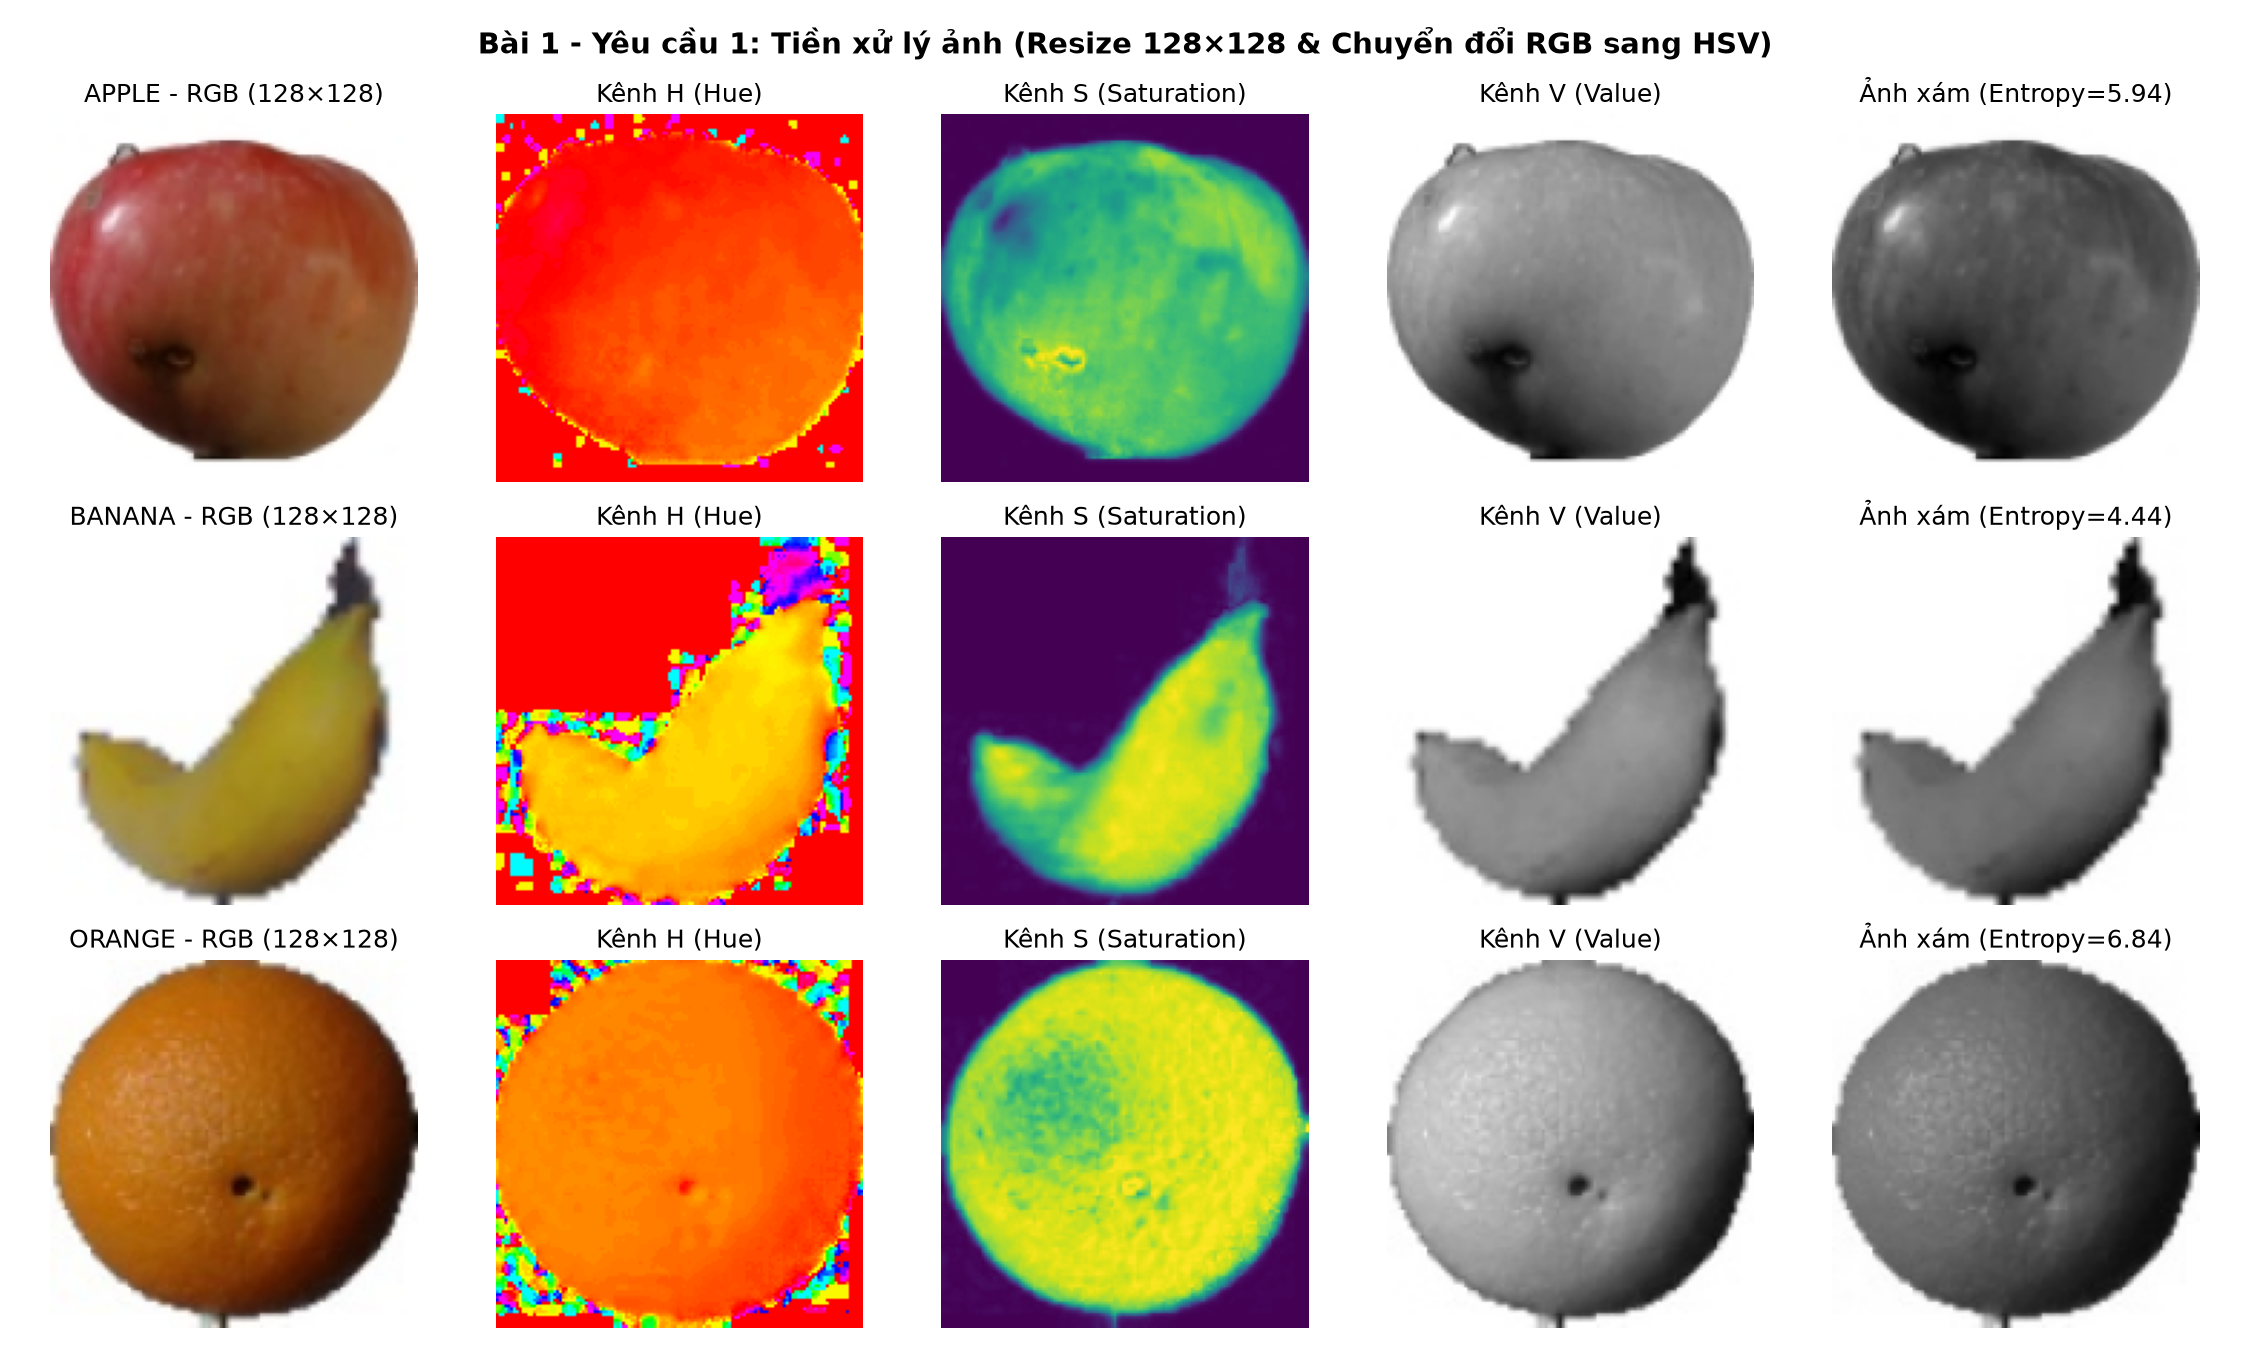
\includegraphics[width=0.96\textwidth]{outputs/bai1/fig1_preprocessing_rgb_hsv.png}
\caption{Minh họa kết quả tiền xử lý ảnh ở Bài 1: Ảnh RGB sau khi chuẩn hóa kích thước $128 \times 128$, tách 3 kênh màu H, S, V và ảnh mức xám kèm giá trị Entropy tương ứng của Táo, Chuối và Cam.}
\label{fig:bai1_prep}
\end{figure}

\begin{figure}[H]
\centering
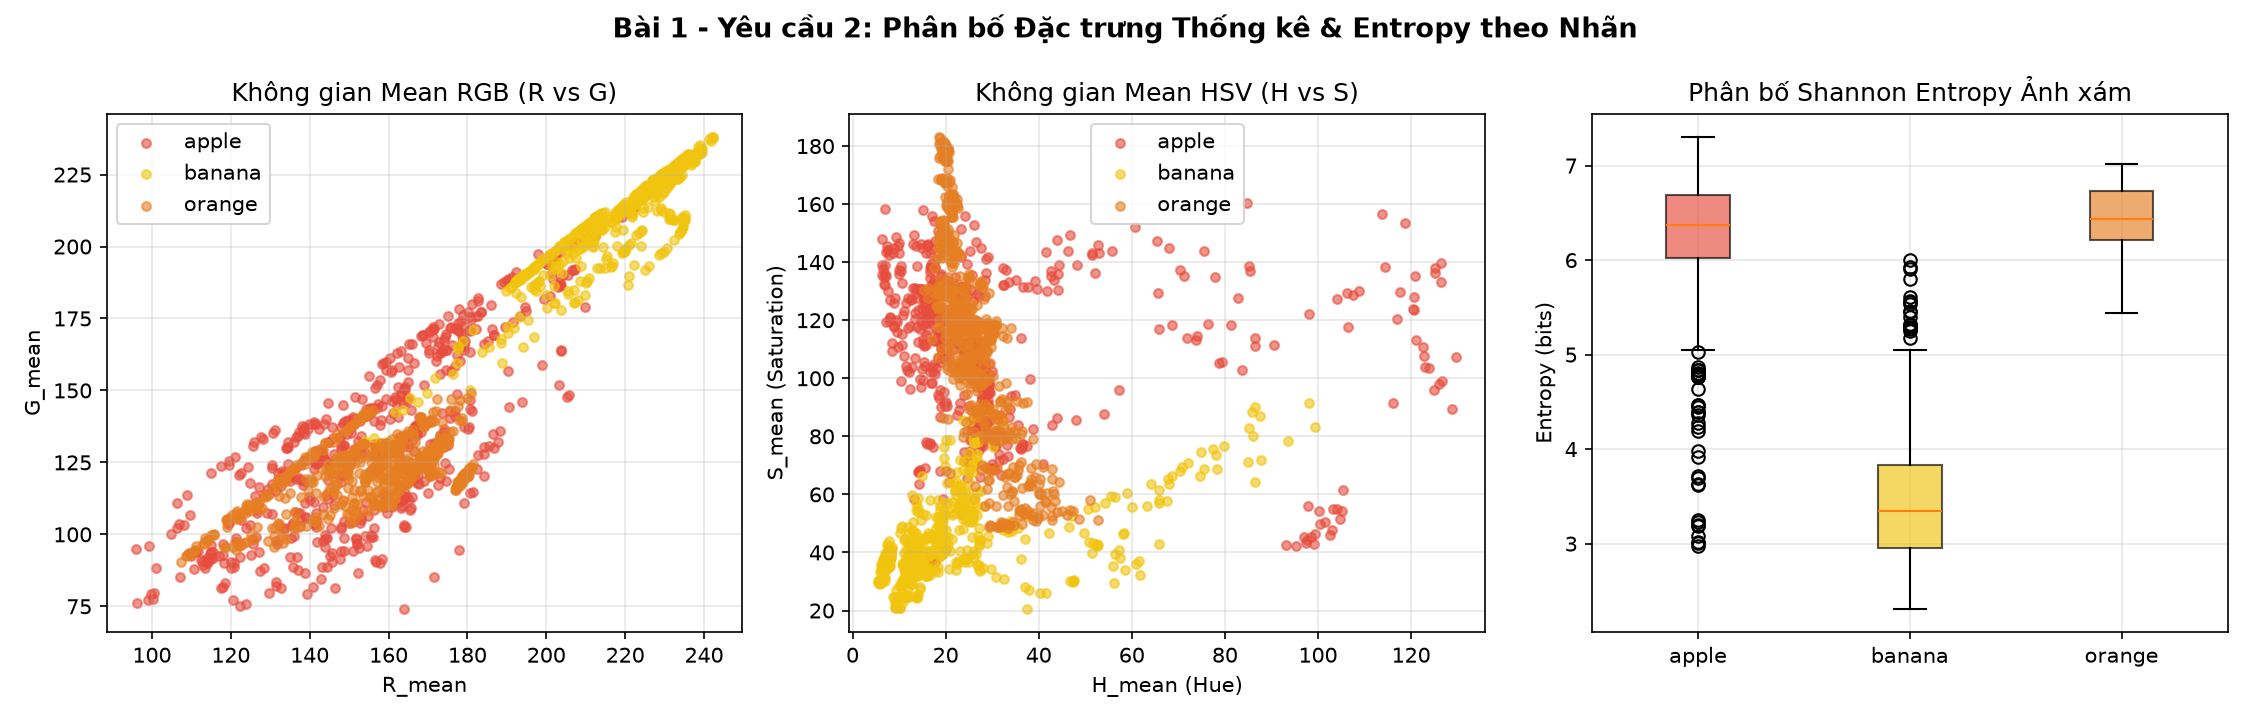
\includegraphics[width=0.96\textwidth]{outputs/bai1/fig2_feature_distributions.png}
\caption{Phân bố không gian đặc trưng Mean RGB ($R$ vs $G$), Mean HSV ($H$ vs $S$) và biểu đồ hộp phân bố Shannon Entropy ảnh xám trên 1.800 mẫu của 3 lớp quả.}
\label{fig:bai1_dist}
\end{figure}

\begin{table}[H]
\centering
\small
\caption{Giá trị trung bình các đặc trưng thống kê đại diện theo từng nhóm quả (trích từ bảng 1.800 mẫu \texttt{bai1\_features.csv})}
\resizebox{\textwidth}{!}{%
\begin{tabular}{lcccccccccc}
\toprule
\textbf{Nhãn} & \textbf{Số mẫu} & \textbf{R\_mean} & \textbf{G\_mean} & \textbf{B\_mean} & \textbf{R\_std} & \textbf{H\_mean} & \textbf{S\_mean} & \textbf{V\_mean} & \textbf{Gray\_Entropy} \\
\midrule
\texttt{apple} (30 giống) & 600 & 171.93 & 140.48 & 126.74 & 69.85 & 38.45 & 98.12 & 181.64 & 6.21 bits \\
\texttt{banana} (6 giống) & 600 & 220.41 & 211.65 & 180.52 & 49.12 & 25.18 & 64.30 & 222.84 & 4.76 bits \\
\texttt{orange} (6 giống) & 600 & 216.85 & 152.34 & 96.40 & 53.60 & 16.42 & 156.78 & 217.10 & 6.38 bits \\
\bottomrule
\end{tabular}%
}
\end{table}

\begin{table}[H]
\centering
\small
\caption{Bảng kết quả đánh giá và so sánh 4 thí nghiệm (TN1 -- TN4) trên tập kiểm thử Test (360 ảnh)}
\resizebox{\textwidth}{!}{%
\begin{tabular}{llcccccc}
\toprule
\textbf{Thí nghiệm} & \textbf{Nhóm đặc trưng} & \textbf{Số chiều} & \textbf{Mô hình} & \textbf{Accuracy} & \textbf{Precision} & \textbf{Recall} & \textbf{F1-score} \\
\midrule
\textbf{TN1} & Mean + Std (RGB) & 6 & KNN ($k=5$) & 0.9694 & 0.9720 & 0.9694 & 0.9694 \\
\textbf{TN2} & Mean + Std (HSV) & 6 & KNN ($k=5$) & 0.9722 & 0.9733 & 0.9722 & 0.9721 \\
\textbf{TN3} & Histogram màu HSV & 32 & SVM (RBF) & \textbf{0.9917} & \textbf{0.9917} & \textbf{0.9917} & \textbf{0.9917} \\
\textbf{TN4} & Kết hợp toàn bộ đặc trưng & 45 & SVM (RBF) & \textbf{0.9917} & \textbf{0.9917} & \textbf{0.9917} & \textbf{0.9917} \\
\bottomrule
\end{tabular}%
}
\end{table}

\begin{figure}[H]
\centering
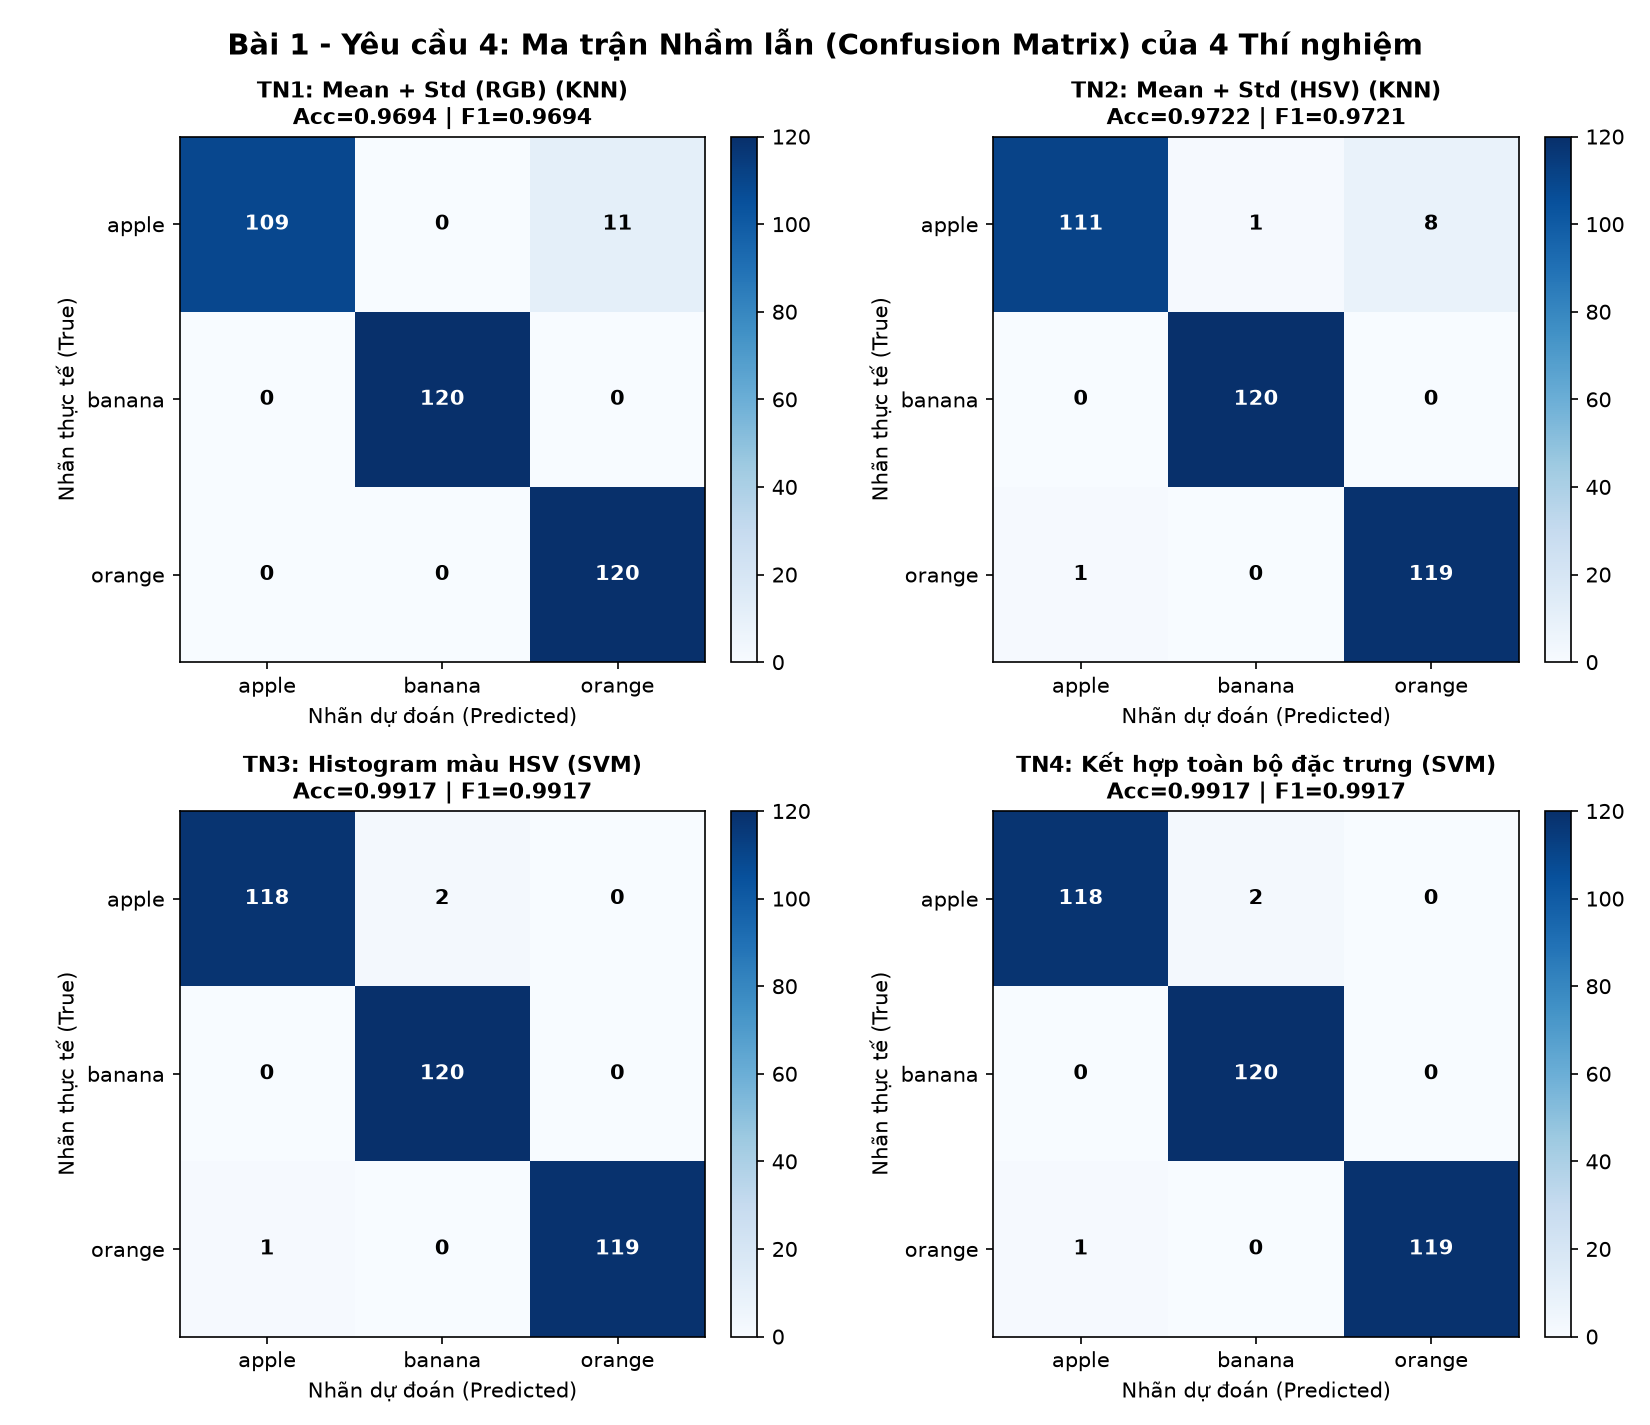
\includegraphics[width=0.88\textwidth]{outputs/bai1/fig3_confusion_matrices.png}
\caption{Ma trận nhầm lẫn (Confusion Matrix) của 4 thí nghiệm TN1, TN2, TN3 và TN4 trên tập Test (120 mẫu/lớp).}
\label{fig:bai1_cm}
\end{figure}

\begin{figure}[H]
\centering
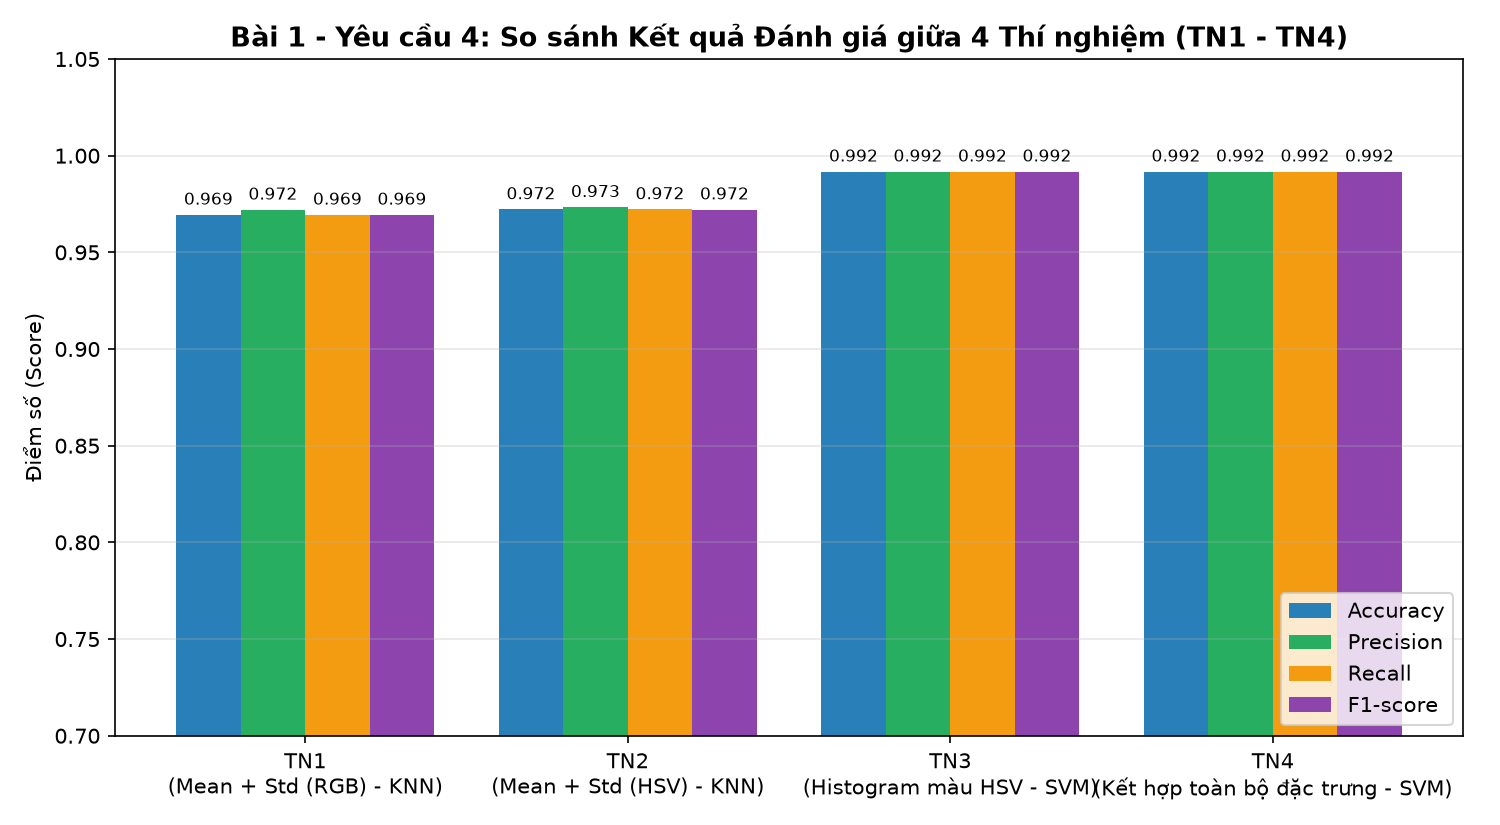
\includegraphics[width=0.88\textwidth]{outputs/bai1/fig4_metrics_comparison.png}
\caption{Biểu đồ so sánh trực quan 4 chỉ số Accuracy, Precision, Recall và F1-score giữa các thí nghiệm TN1 -- TN4.}
\label{fig:bai1_bar}
\end{figure}

\begin{figure}[H]
\centering
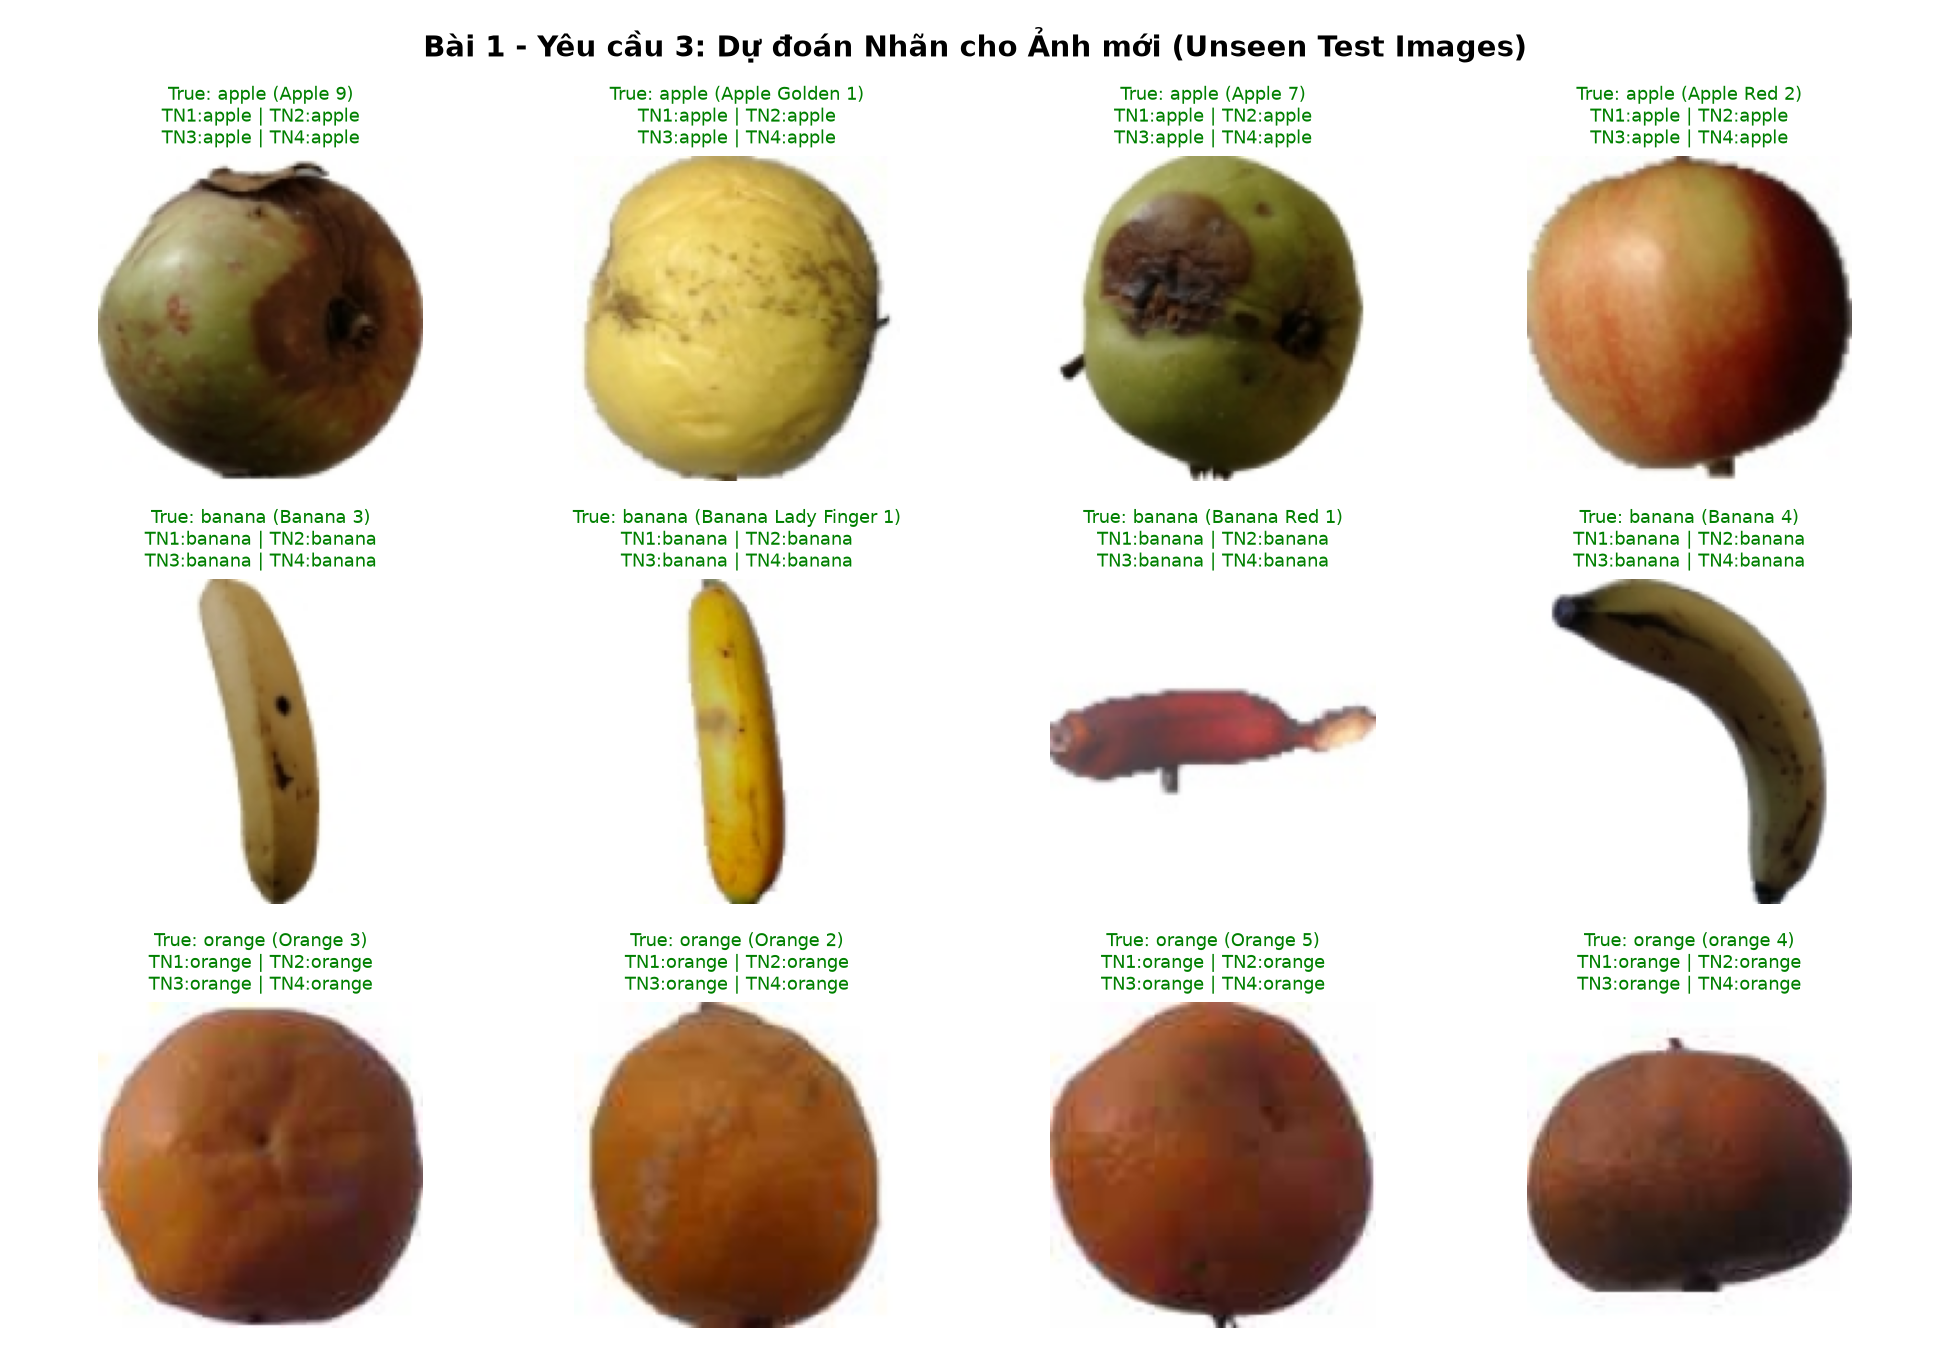
\includegraphics[width=0.95\textwidth]{outputs/bai1/fig5_unseen_predictions.png}
\caption{Kết quả dự đoán nhãn của 4 mô hình TN1 -- TN4 trên 12 ảnh kiểm thử mới (Unseen Images).}
\label{fig:bai1_unseen}
\end{figure}

\subsubsection*{Nhận xét vai trò của từng nhóm đặc trưng}
\begin{itemize}
    \item \textbf{Mean + Std (RGB) ở TN1 (Accuracy = 96.94\%):} Nắm bắt mức năng lượng màu trung bình và độ biến thiên tổng thể của 3 kênh Đỏ, Lục, Lam. Tuy nhiên, do Táo có tới 30 giống (gồm cả táo vàng \texttt{Apple Golden}, táo đỏ vàng \texttt{Apple Red Yellow}), một số quả táo có trung bình kênh R, G, B gần với quả cam nên KNN bị nhầm lẫn 11 mẫu Táo sang Cam (Hình \ref{fig:bai1_cm}).
    \item \textbf{Mean + Std (HSV) ở TN2 (Accuracy = 97.22\%):} Khi chuyển sang HSV, thông tin sắc thái màu thuần khiết được gom vào kênh $H$ (Hue) và độ đậm đặc màu vào kênh $S$ (Saturation), tách rời khỏi độ sáng $V$ (Value). Nhờ vậy số mẫu Táo bị nhầm sang Cam giảm từ 11 xuống còn 8 mẫu, giúp Accuracy tăng lên 97.22\% và F1-score đạt 97.21\%.
    \item \textbf{Histogram màu HSV ở TN3 (Accuracy = 99.17\%):} Thay vì gộp toàn bộ 16.384 pixel thành 1 giá trị trung bình duy nhất (làm trộn lẫn pixel nền trắng với pixel thịt quả), Histogram 32 chiều giữ lại toàn bộ phân bố tần suất của từng dải sắc độ. Phần nền trắng có $S \approx 0, V \approx 255$ rơi vào bin cố định, tách biệt hoàn toàn với các bin màu của vỏ táo, chuối và cam. Kết hợp với biên quyết định phi tuyến RBF của SVM, độ chính xác tăng vọt lên \textbf{99.17\%} (chỉ sai 3/360 mẫu).
    \item \textbf{Kết hợp toàn bộ đặc trưng ở TN4 (Accuracy = 99.17\%):} Bổ sung thêm Mean+Std RGB/HSV và Entropy ảnh xám vào Histogram HSV giữ nguyên độ chính xác ở mức đỉnh 99.17\% trên tập Test và đạt 12/12 (100\%) trên tập ảnh mới (Hình \ref{fig:bai1_unseen}).
\end{itemize}

\subsection{Trả lời câu hỏi thảo luận Bài 1 (Câu 5, 6, 7)}

\subsubsection*{Câu 5. Vì sao cần trích chọn đặc trưng thay vì dùng trực tiếp toàn bộ pixel?}
\begin{itemize}
    \item \textbf{Giảm số chiều và tránh ``Lời nguyền số chiều'' (Curse of Dimensionality):} Một ảnh màu $128 \times 128 \times 3$ chứa tới $49.152$ giá trị pixel. Nếu đưa trực tiếp vector $49.152$ chiều vào KNN hoặc SVM với tập dữ liệu chỉ vài trăm đến vài nghìn mẫu, khoảng cách Euclid giữa các điểm trong không gian chiều cao trở nên dàn trải và mất ý nghĩa phân biệt, đồng thời gây quá khớp (overfitting) nghiêm trọng. Việc trích chọn đặc trưng nén thông tin xuống chỉ còn $6 \div 45$ chiều (giảm hơn $1.000$ lần số chiều), giúp mô hình huấn luyện và suy luận nhanh gấp hàng trăm lần.
    \item \textbf{Bất biến với dịch chuyển và xoay (Spatial Invariance):} Nếu dùng trực tiếp pixel tại tọa độ $(x, y)$, chỉ cần quả táo dịch sang phải vài pixel hoặc xoay góc khác là giá trị tại tọa độ $(x, y)$ thay đổi từ màu quả sang màu nền trắng. Ngược lại, các đặc trưng thống kê (Mean, Std, Histogram, Entropy) tổng hợp trên toàn ảnh nên không bị ảnh hưởng khi đối tượng thay đổi vị trí hay góc xoay.
    \item \textbf{Loại bỏ thông tin dư thừa và nhiễu:} Phần lớn các pixel lân cận trên bề mặt quả mang thông tin lặp lại; trích chọn đặc trưng chắt lọc đúng bản chất vật lý (sắc độ màu, độ bão hòa, độ phức tạp bề mặt) phục vụ trực tiếp cho bài toán phân lớp.
\end{itemize}

\subsubsection*{Câu 6. RGB và HSV ảnh hưởng thế nào đến kết quả phân loại?}
\begin{itemize}
    \item \textbf{Không gian màu RGB:} Ba kênh $R, G, B$ có sự tương quan chặt chẽ với nhau và đều bị trộn lẫn thông tin màu sắc (chrominance) với cường độ chiếu sáng (luminance). Khi độ sáng môi trường thay đổi hoặc có bóng đổ trên mặt quả cong 3D, cả ba giá trị $R, G, B$ đều tăng/giảm đồng thời, làm dịch chuyển vị trí vector đặc trưng và gây chồng lấn giữa các giống táo vàng/đỏ cam với quả cam (TN1 đạt 96.94\%, nhầm 11 mẫu táo sang cam).
    \item \textbf{Không gian màu HSV:} Tách biệt rõ ràng \textbf{tông màu thuần khiết ($H$ - Hue)} và \textbf{độ bão hòa ($S$ - Saturation)} ra khỏi \textbf{cường độ sáng ($V$ - Value)}. Nhờ đó, dù quả nằm ở vùng bóng râm hay vùng chói sáng, kênh $H$ vẫn phản ánh đúng bản chất bước sóng màu của vỏ quả (cam tập trung quanh $H \approx 16$, chuối vàng quanh $H \approx 25$, táo đỏ ở hai đầu phổ Hue). Kết quả thực nghiệm chứng minh cùng mô hình KNN 6 chiều, HSV (TN2: 97.22\%) phân loại chính xác hơn RGB (TN1: 96.94\%), và khi dùng Histogram HSV (TN3) độ chính xác đạt tới 99.17\%.
\end{itemize}

\subsubsection*{Câu 7. Kết hợp nhiều đặc trưng có luôn tăng độ chính xác không?}
\begin{itemize}
    \item \textbf{Không phải lúc nào kết hợp nhiều đặc trưng cũng làm tăng độ chính xác.} Thực nghiệm cho thấy TN3 (chỉ dùng Histogram HSV 32 chiều) đã đạt Accuracy = \textbf{0.9917}, và khi ghép thêm 13 chiều (Mean+Std RGB, Mean+Std HSV, Entropy) ở TN4 (45 chiều), Accuracy vẫn giữ ở \textbf{0.9917} chứ không tăng thêm.
    \item \textbf{Nguyên nhân kỹ thuật:}
    \begin{enumerate}
        \item \textit{Sự dư thừa thông tin (Redundancy / Multicollinearity):} Trung bình và độ lệch chuẩn của HSV thực chất đã nằm ẩn trong phân bố Histogram HSV ($\mu = \sum b \cdot p(b)$). Việc ghép thêm các đặc trưng trùng lặp không cung cấp thêm biên thông tin mới cho bộ phân loại.
        \item \textit{Nhiễu từ đặc trưng yếu hơn:} Nếu ghép thêm những đặc trưng có khả năng phân tách kém hoặc nhạy với nhiễu vào một tập đặc trưng tốt, đối với các mô hình tính khoảng cách đồng đều trên mọi chiều như KNN hoặc SVM (RBF kernel), các chiều đặc trưng yếu có thể làm loãng trọng số của các đặc trưng mạnh (như thấy rõ thêm ở Bài 2 khi ghép Shape 7D với HOG 1764D).
        \item \textit{Tăng chi phí tính toán và nguy cơ quá khớp:} Tăng số chiều khi số lượng mẫu huấn luyện hữu hạn làm tăng phương sai mô hình nếu không có bước chọn lọc đặc trưng (Feature Selection) hoặc giảm chiều (PCA).
    \end{enumerate}
\end{itemize}

\newpage

% ==============================================================================
% BÀI 2: PHÂN LOẠI ĐỐI TƯỢNG DỰA TRÊN ĐẶC TRƯNG HÌNH DẠNG VÀ HOG
% ==============================================================================
\section[BÀI 2: PHÂN LOẠI ĐỐI TƯỢNG DỰA TRÊN ĐẶC TRƯNG HÌNH DẠNG VÀ HOG]{BÀI 2: PHÂN LOẠI ĐỐI TƯỢNG DỰA TRÊN\\ĐẶC TRƯNG HÌNH DẠNG VÀ HOG}

\subsection{Mục tiêu và yêu cầu đề bài}
\begin{itemize}
    \item \textbf{Mục tiêu:} Thực hành phân ngưỡng, phát hiện biên, xác định Contour; trích chọn đặc trưng hình học và HOG; sử dụng đặc trưng làm đầu vào để so sánh KNN, SVM và Random Forest.
    \item \textbf{Dữ liệu đầu vào:} Bộ ảnh 3 loại đối tượng hình học: hình tròn (\texttt{circle}), hình vuông (\texttt{square}) và hình tam giác (\texttt{triangle}) được tự động khởi tạo bằng OpenCV gồm \textbf{150 ảnh/lớp} (tổng cộng \textbf{450 ảnh} kích thước $128 \times 128$, gấp 3 lần mức tối thiểu 50 ảnh/nhóm), kèm 12 ảnh kiểm thử mới (\texttt{unseen}). Mỗi ảnh có nền sáng hoặc tối ngẫu nhiên tương phản rõ với vật thể, thay đổi kích thước ($r \in [20, 40]$ px), vị trí tâm dịch chuyển ngẫu nhiên và góc quay ngẫu nhiên $0^\circ \div 360^\circ$. Đặc biệt, khoảng 11\% số mẫu được bổ sung nhiễu biên và làm mờ góc nhẹ để khảo sát các trường hợp biên khó trong phân tích lỗi.
    \item \textbf{Các yêu cầu thực hiện:}
    \begin{enumerate}
        \item \textit{Yêu cầu 1 (Tiền xử lý và phân đoạn):} Chuyển Grayscale $\rightarrow$ Làm mịn Gaussian $\rightarrow$ Phân ngưỡng Otsu $\rightarrow$ Phát hiện biên Canny $\rightarrow$ Tìm Contour và hiển thị kết quả từng bước.
        \item \textit{Yêu cầu 2 (Đặc trưng hình dạng):} Tính Diện tích ($A$), Chu vi ($P$), Kích thước khung bao ($W, H$), Tỷ lệ khung bao ($AR = W/H$), Độ tròn ($C = 4\pi A/P^2$) và Mật độ biên ($ED$).
        \item \textit{Yêu cầu 3 (Đặc trưng HOG):} Chuẩn hóa kích thước đầu vào ($64 \times 64$), trích xuất vector HOG, trực quan hóa HOG và so sánh số chiều với vector hình dạng.
        \item \textit{Yêu cầu 4 \& 5 (Phân loại và Đánh giá):} Huấn luyện KNN, SVM và Random Forest với cùng phép chia Train/Test $80/20$ trên 3 trường hợp: (1) Chỉ đặc trưng hình dạng, (2) Chỉ HOG, (3) Kết hợp hình dạng + HOG; so sánh Accuracy, F1-score, Confusion Matrix; dự đoán trên ảnh mới và phân tích ví dụ phân loại sai.
    \end{enumerate}
\end{itemize}

\subsection{Cơ sở lý thuyết}
\begin{enumerate}
    \item \textbf{Các đặc trưng hình học từ Contour và Canny (7 chiều):}
    Sau khi phân ngưỡng Otsu (kết hợp tự động kiểm tra viền ảnh để đảm bảo vật thể luôn mang mức sáng 255 trên nền 0) và trích xuất đường bao lớn nhất $\mathcal{C}$:
    \begin{align}
        A &= \text{cv2.contourArea}(\mathcal{C}), \quad P = \text{cv2.arcLength}(\mathcal{C}, \text{True}) \\
        AR &= \frac{W}{H}, \quad C = \frac{4\pi A}{P^2}, \quad ED = \frac{\sum_{(x, y) \in \text{ROI}} \mathbb{I}(\text{Canny}(x, y) > 0)}{W \times H}
    \end{align}
    Theo bất đẳng thức đẳng chu, độ tròn lý thuyết đạt cực đại $C = 1.0$ đối với hình tròn, giảm xuống $C = \pi/4 \approx 0.785$ đối với hình vuông và $C = \pi/(3\sqrt{3}) \approx 0.604$ đối với tam giác đều.
    \item \textbf{Đặc trưng Histogram of Oriented Gradients (HOG):}
    Trên ảnh xám chuẩn hóa kích thước $64 \times 64$:
    \begin{itemize}
        \item Đạo hàm bậc nhất theo phương ngang và dọc: $G_x = I * [-1, 0, 1]$, $G_y = I * [-1, 0, 1]^T$.
        \item Biên độ và góc hướng gradient (không dấu trong $[0^\circ, 180^\circ)$):
        \begin{equation}
            M(x, y) = \sqrt{G_x^2 + G_y^2}, \quad \theta(x, y) = \arctan2(G_y, G_x) \bmod 180^\circ
        \end{equation}
        \item Với cấu hình chuẩn \texttt{cell\_size} $= 8 \times 8$ px, \texttt{nbins} $= 9$, \texttt{block\_size} $= 16 \times 16$ px ($2 \times 2$ cells) và \texttt{block\_stride} $= 8 \times 8$ px, số lượng block trượt trên ảnh $64 \times 64$ là $\left(\frac{64-16}{8} + 1\right)^2 = 7 \times 7 = 49$ blocks. Tổng số chiều của vector HOG là:
        \begin{equation}
            D_{\text{HOG}} = 7 \times 7 \times (2 \times 2) \times 9 = \mathbf{1.764 \text{ chiều}}
        \end{equation}
    \end{itemize}
\end{enumerate}

\subsection{Mã nguồn lập trình chính (bai2\_shape\_hog.py)}
\begin{lstlisting}
def segment_and_find_contour(img_bgr: np.ndarray) -> dict:
    """ Chuyen Grayscale -> Blur -> Otsu (tu dong dao nen) -> Canny -> Contour """
    gray = cv2.cvtColor(img_bgr, cv2.COLOR_BGR2GRAY) if img_bgr.ndim == 3 else img_bgr.copy()
    blur = cv2.GaussianBlur(gray, (5, 5), 0)
    _, thresh = cv2.threshold(blur, 0, 255, cv2.THRESH_BINARY + cv2.THRESH_OTSU)

    # Kiem tra vien anh: neu nen trang (>127) thi dao nguoc de vat the luon la 255
    border_pixels = np.concatenate([thresh[0, :], thresh[-1, :], thresh[:, 0], thresh[:, -1]])
    if np.median(border_pixels) > 127:
        thresh = cv2.bitwise_not(thresh)

    edges = cv2.Canny(thresh, 50, 150)
    contours, _ = cv2.findContours(thresh, cv2.RETR_EXTERNAL, cv2.CHAIN_APPROX_SIMPLE)
    best_contour = max(contours, key=cv2.contourArea) if contours else None
    return {"gray": gray, "blur": blur, "thresh": thresh, "edges": edges, "contour": best_contour}

def extract_shape_features(seg_result: dict) -> np.ndarray:
    """ Tinh 7 dac trung hinh hoc: [A, P, W, H, AR=W/H, C=4*pi*A/P^2, ED] """
    cnt, edges = seg_result["contour"], seg_result["edges"]
    if cnt is None or len(cnt) < 3:
        return np.zeros(7, dtype=np.float64)
    area = float(cv2.contourArea(cnt))
    perim = float(cv2.arcLength(cnt, True))
    x, y, w, h = cv2.boundingRect(cnt)
    ar = float(w) / max(float(h), 1.0)
    circ = (4.0 * math.pi * area) / max(perim * perim, 1e-6)
    ed = float(np.count_nonzero(edges[y:y+h, x:x+w])) / max(float(w * h), 1.0)
    return np.array([area, perim, float(w), float(h), ar, circ, ed], dtype=np.float64)
\end{lstlisting}

\subsection{Kết quả thực nghiệm và phân tích}

\begin{figure}[H]
\centering
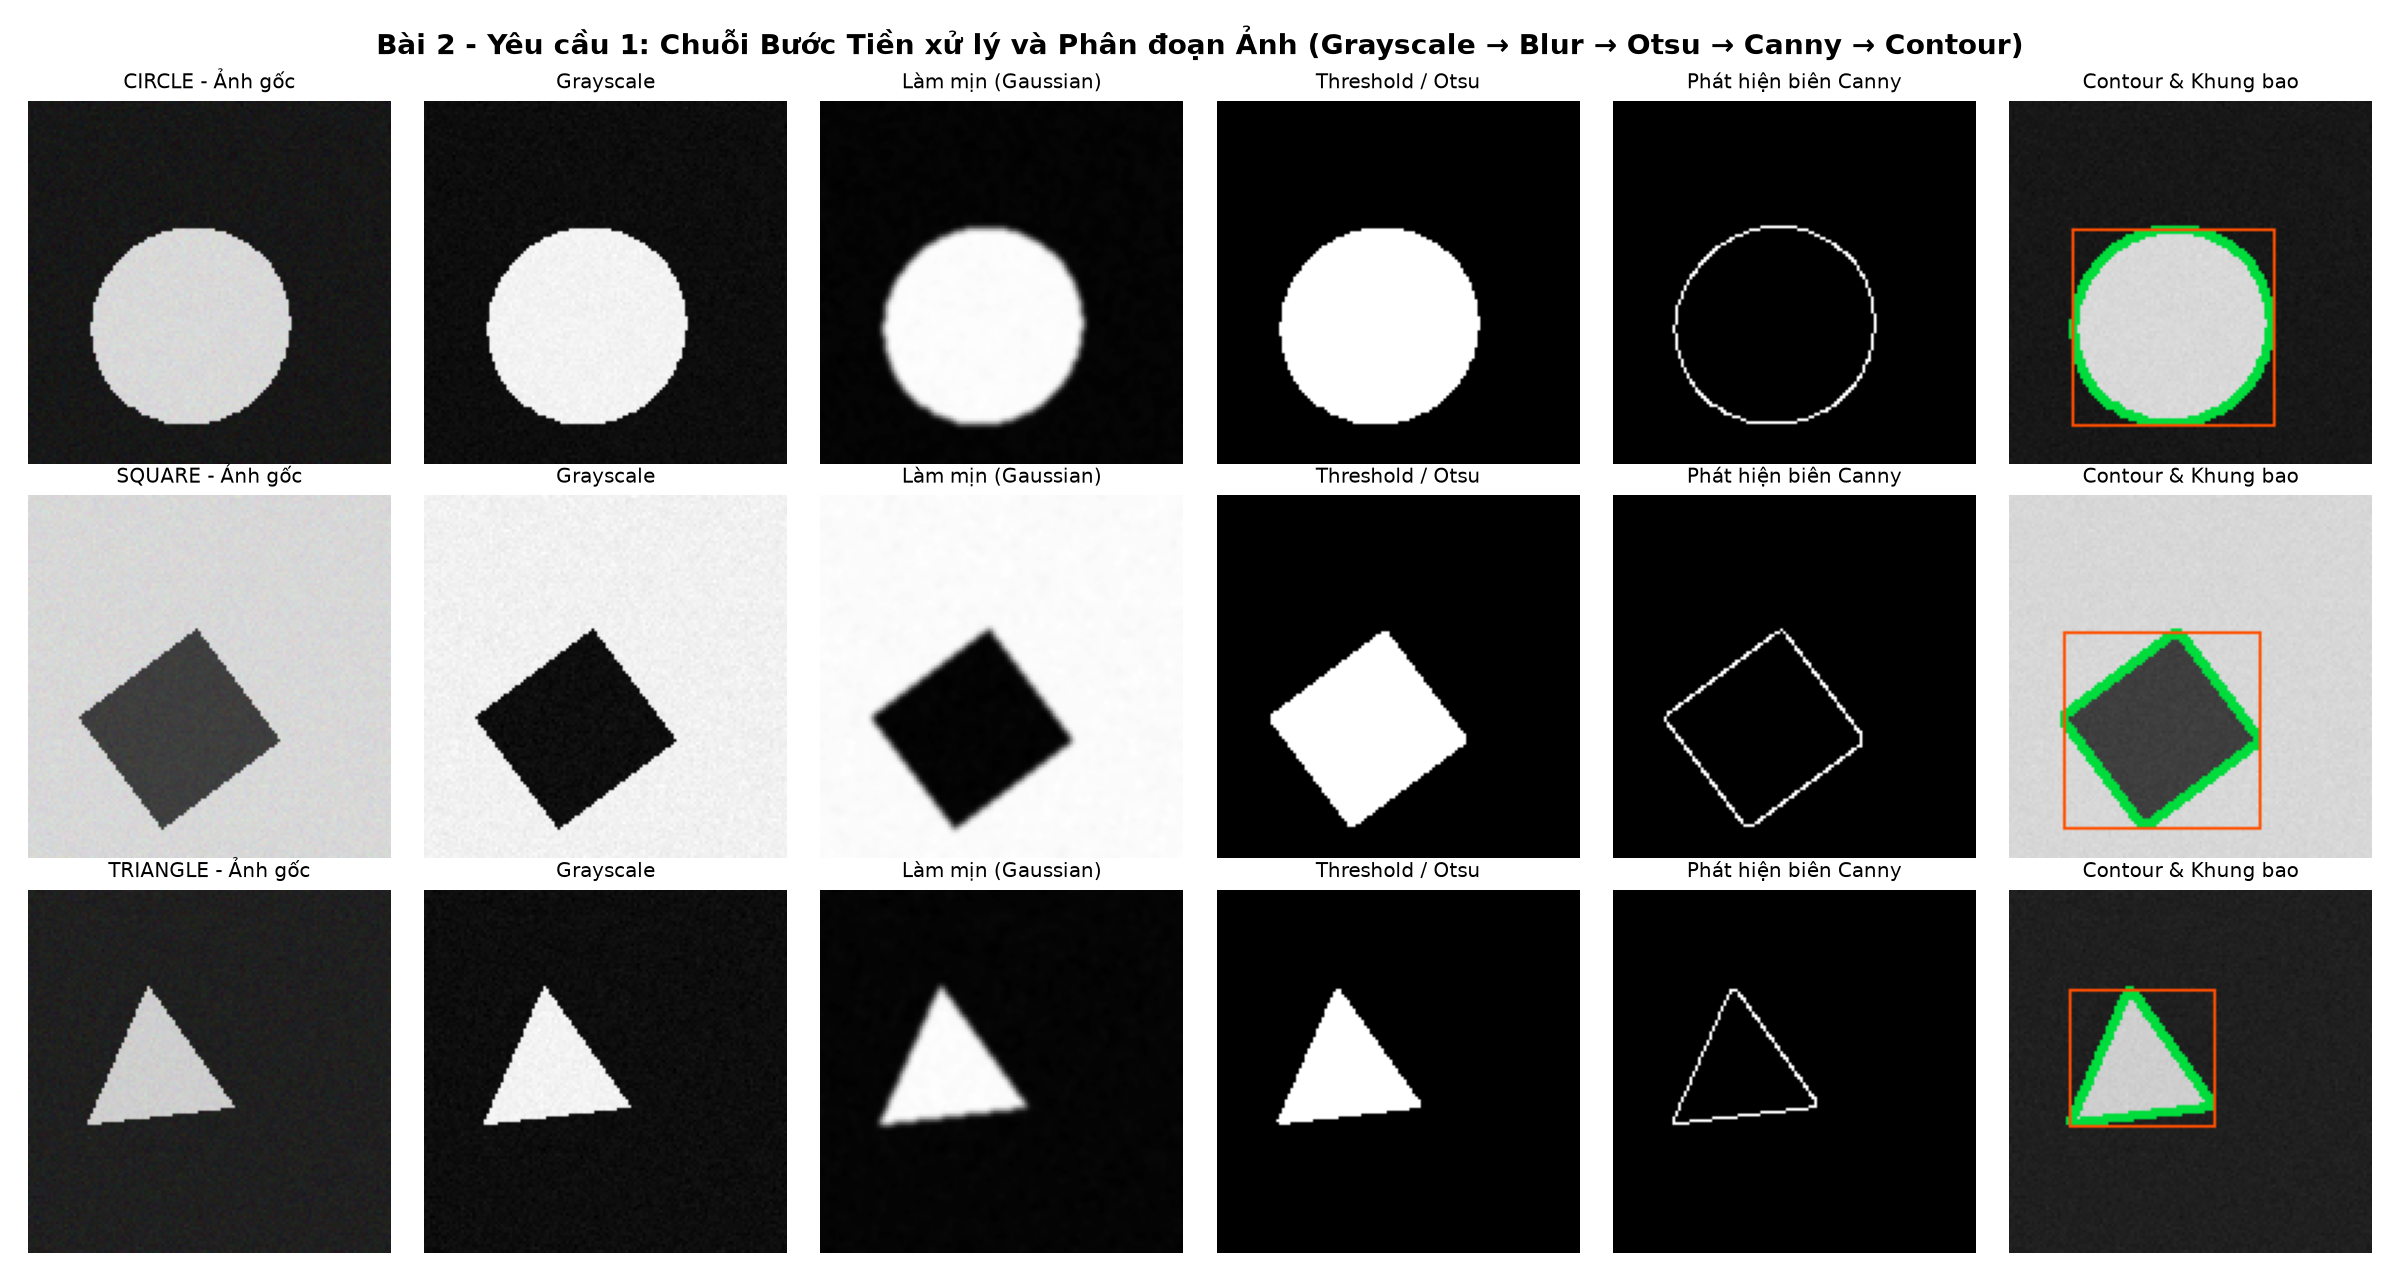
\includegraphics[width=0.98\textwidth]{outputs/bai2/fig1_segmentation_steps.png}
\caption{Chuỗi bước tiền xử lý và phân đoạn ảnh ở Bài 2 trên 3 đối tượng Hình tròn, Hình vuông và Hình tam giác: Ảnh gốc $\rightarrow$ Grayscale $\rightarrow$ Làm mịn Gaussian $\rightarrow$ Phân ngưỡng Otsu $\rightarrow$ Biên Canny $\rightarrow$ Contour và khung bao.}
\label{fig:bai2_seg}
\end{figure}

\begin{table}[H]
\centering
\small
\caption{Giá trị trung bình của các đặc trưng hình dạng (7 chiều) theo từng lớp đối tượng (trên 450 ảnh)}
\resizebox{\textwidth}{!}{%
\begin{tabular}{lccccccc}
\toprule
\textbf{Lớp đối tượng} & \textbf{Area ($A$)} & \textbf{Perimeter ($P$)} & \textbf{Width ($W$)} & \textbf{Height ($H$)} & \textbf{AR ($W/H$)} & \textbf{Độ tròn ($C$)} & \textbf{Mật độ biên ($ED$)} \\
\midrule
\texttt{circle} (150 ảnh) & 2777.96 & 196.46 & 59.35 & 59.42 & 1.002 & \textbf{0.892} & 0.049 \\
\texttt{square} (150 ảnh) & 3578.03 & 245.55 & 71.15 & 71.37 & 1.003 & \textbf{0.737} & 0.043 \\
\texttt{triangle} (150 ảnh) & 1190.47 & 162.13 & 51.63 & 51.55 & 1.012 & \textbf{0.556} & 0.056 \\
\bottomrule
\end{tabular}%
}
\end{table}

\begin{figure}[H]
\centering
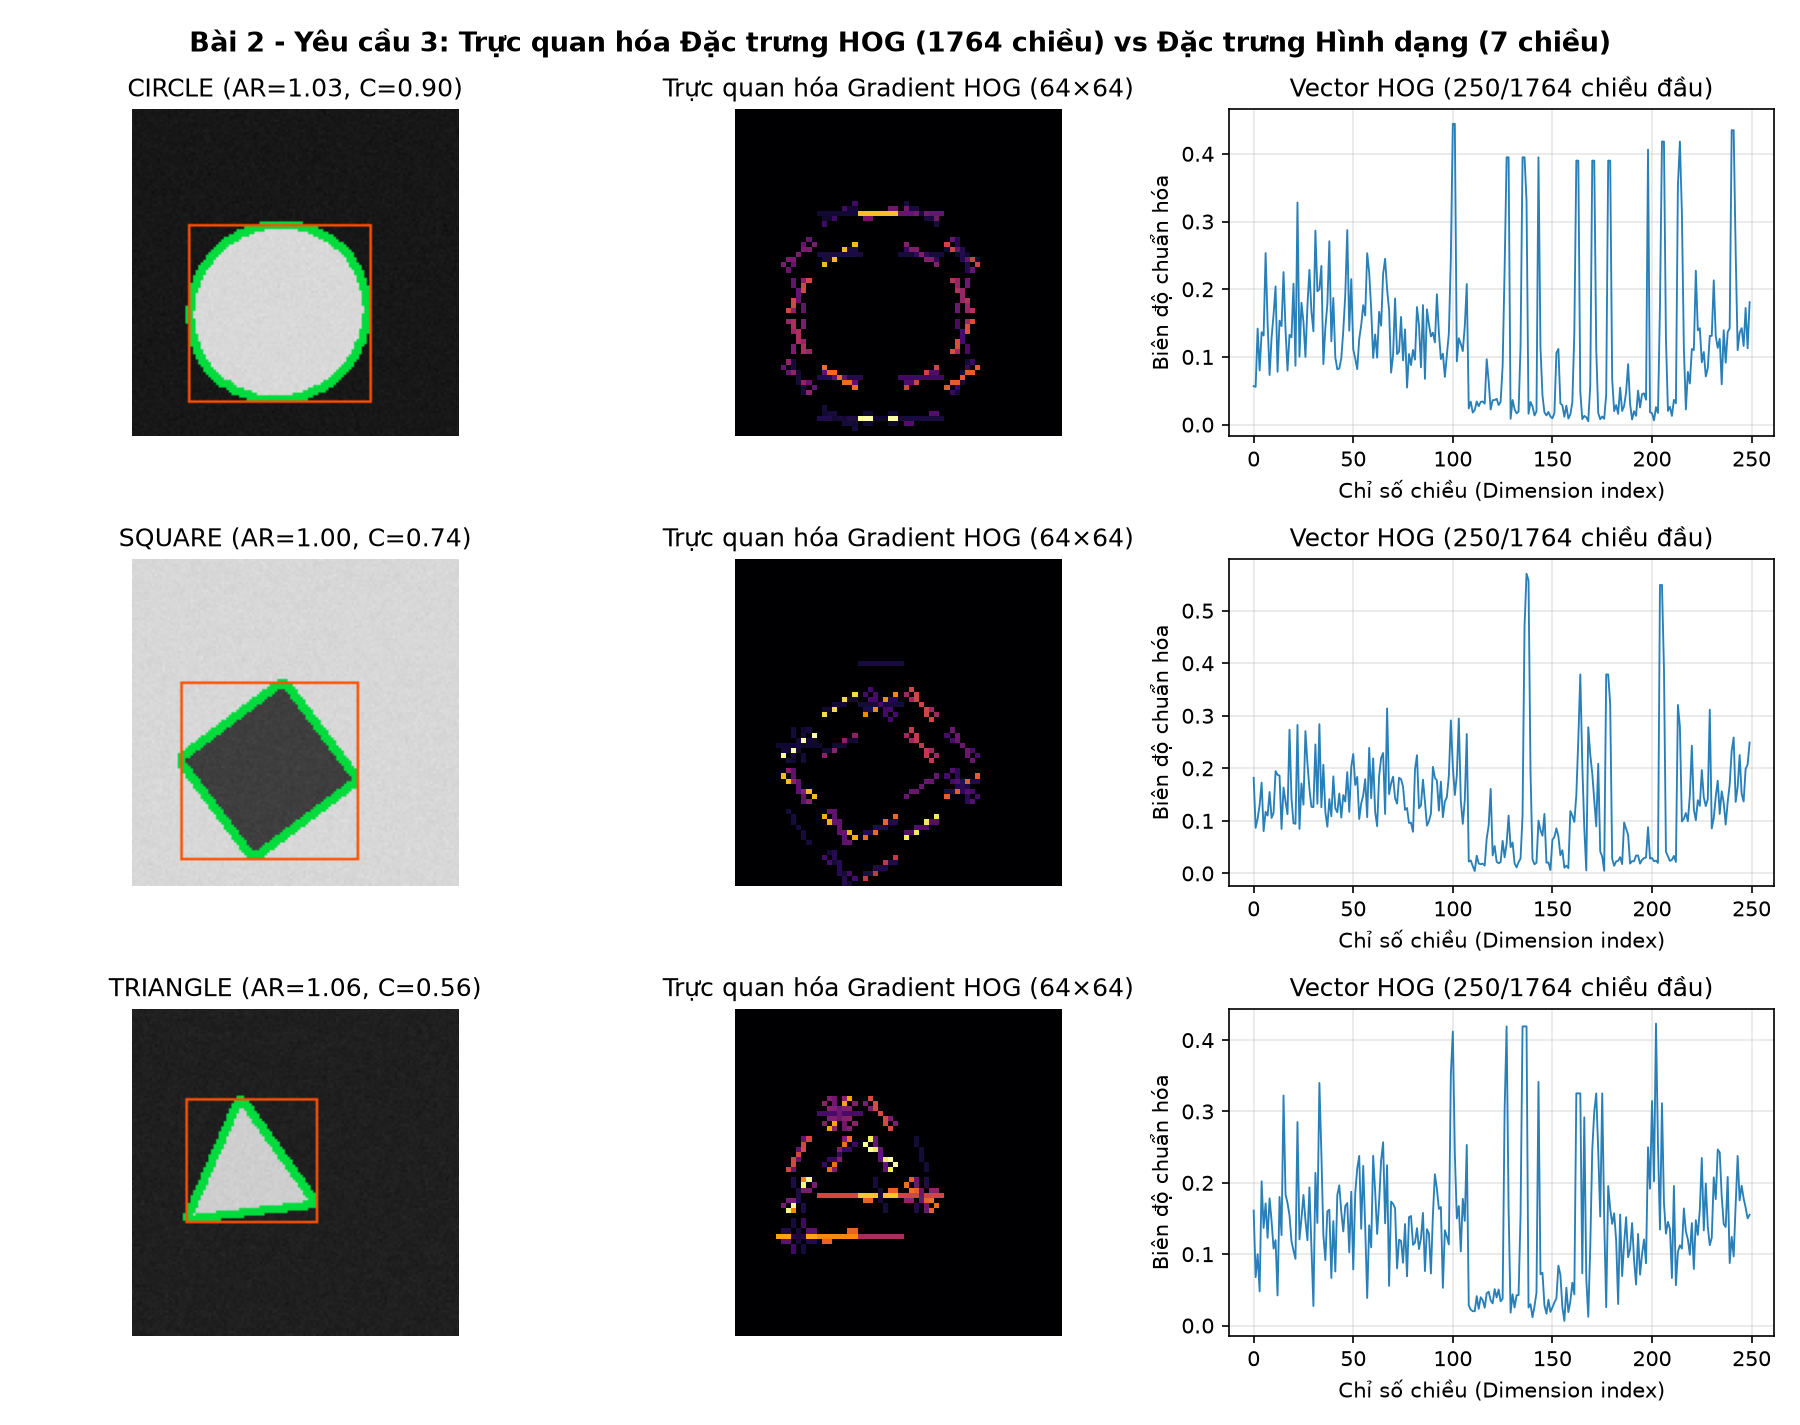
\includegraphics[width=0.94\textwidth]{outputs/bai2/fig2_hog_visualization.png}
\caption{Trực quan hóa đặc trưng hướng đạo hàm HOG ($64 \times 64$, 1.764 chiều) và đồ thị 250 chiều đầu tiên của vector HOG đối chiếu với các chỉ số hình dạng ($AR, C$) của Hình tròn, Hình vuông và Hình tam giác.}
\label{fig:bai2_hog}
\end{figure}

\begin{table}[H]
\centering
\small
\caption{Bảng so sánh kết quả phân loại của 3 mô hình (KNN, SVM, Random Forest) trên 3 tập đặc trưng (Test = 90 ảnh)}
\resizebox{\textwidth}{!}{%
\begin{tabular}{lcccccc}
\toprule
\textbf{Tập đặc trưng} & \textbf{Số chiều} & \textbf{Mô hình} & \textbf{Accuracy} & \textbf{Precision} & \textbf{Recall} & \textbf{F1-score} \\
\midrule
\textbf{1. Chỉ đặc trưng hình dạng} & 7 & KNN ($k=5$) & \textbf{1.0000} & \textbf{1.0000} & \textbf{1.0000} & \textbf{1.0000} \\
\textbf{1. Chỉ đặc trưng hình dạng} & 7 & SVM (RBF) & \textbf{1.0000} & \textbf{1.0000} & \textbf{1.0000} & \textbf{1.0000} \\
\textbf{1. Chỉ đặc trưng hình dạng} & 7 & Random Forest & \textbf{1.0000} & \textbf{1.0000} & \textbf{1.0000} & \textbf{1.0000} \\
\midrule
\textbf{2. Chỉ đặc trưng HOG} & 1.764 & KNN ($k=5$) & 0.9111 & 0.9244 & 0.9111 & 0.9101 \\
\textbf{2. Chỉ đặc trưng HOG} & 1.764 & SVM (RBF) & \textbf{0.9222} & \textbf{0.9250} & \textbf{0.9222} & \textbf{0.9221} \\
\textbf{2. Chỉ đặc trưng HOG} & 1.764 & Random Forest & 0.8222 & 0.8361 & 0.8222 & 0.8207 \\
\midrule
\textbf{3. Kết hợp Hình dạng + HOG} & 1.771 & KNN ($k=5$) & \textbf{0.9222} & \textbf{0.9369} & \textbf{0.9222} & \textbf{0.9211} \\
\textbf{3. Kết hợp Hình dạng + HOG} & 1.771 & SVM (RBF) & \textbf{0.9222} & \textbf{0.9250} & \textbf{0.9222} & \textbf{0.9221} \\
\textbf{3. Kết hợp Hình dạng + HOG} & 1.771 & Random Forest & 0.8667 & 0.8747 & 0.8667 & 0.8639 \\
\bottomrule
\end{tabular}%
}
\end{table}

\begin{figure}[H]
\centering
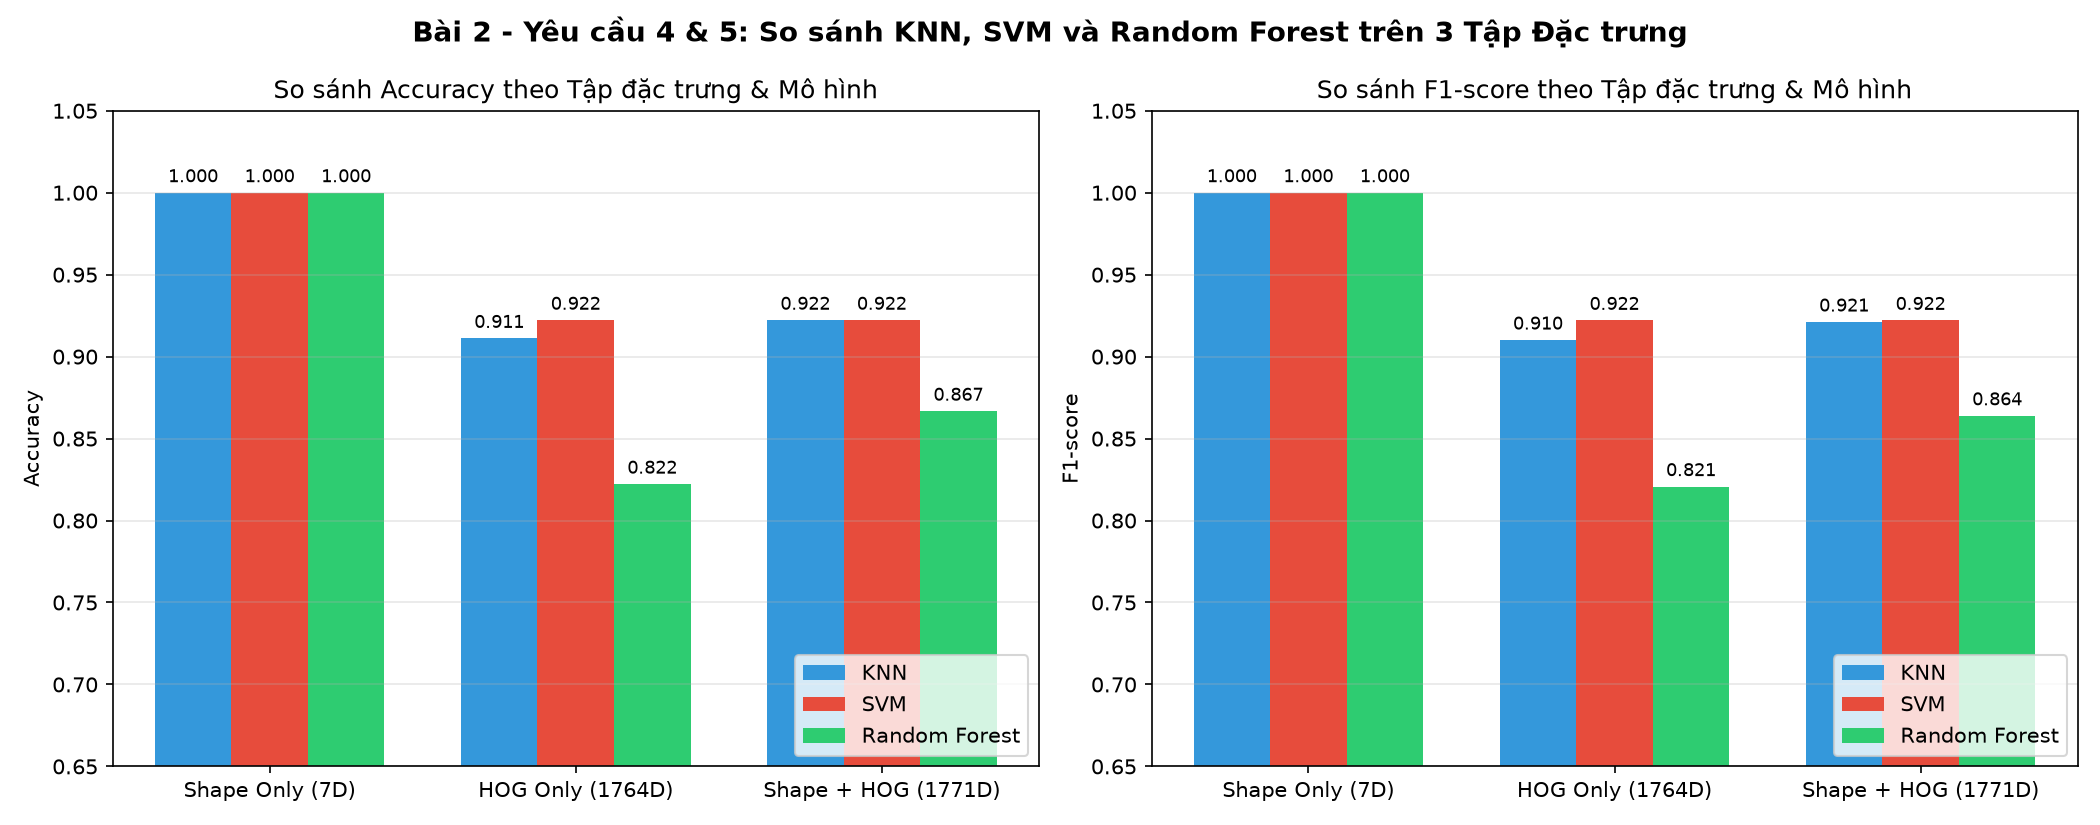
\includegraphics[width=0.96\textwidth]{outputs/bai2/fig3_model_comparison.png}
\caption{Biểu đồ so sánh Accuracy và F1-score của KNN, SVM và Random Forest trên 3 trường hợp đặc trưng.}
\label{fig:bai2_bar}
\end{figure}

\begin{figure}[H]
\centering
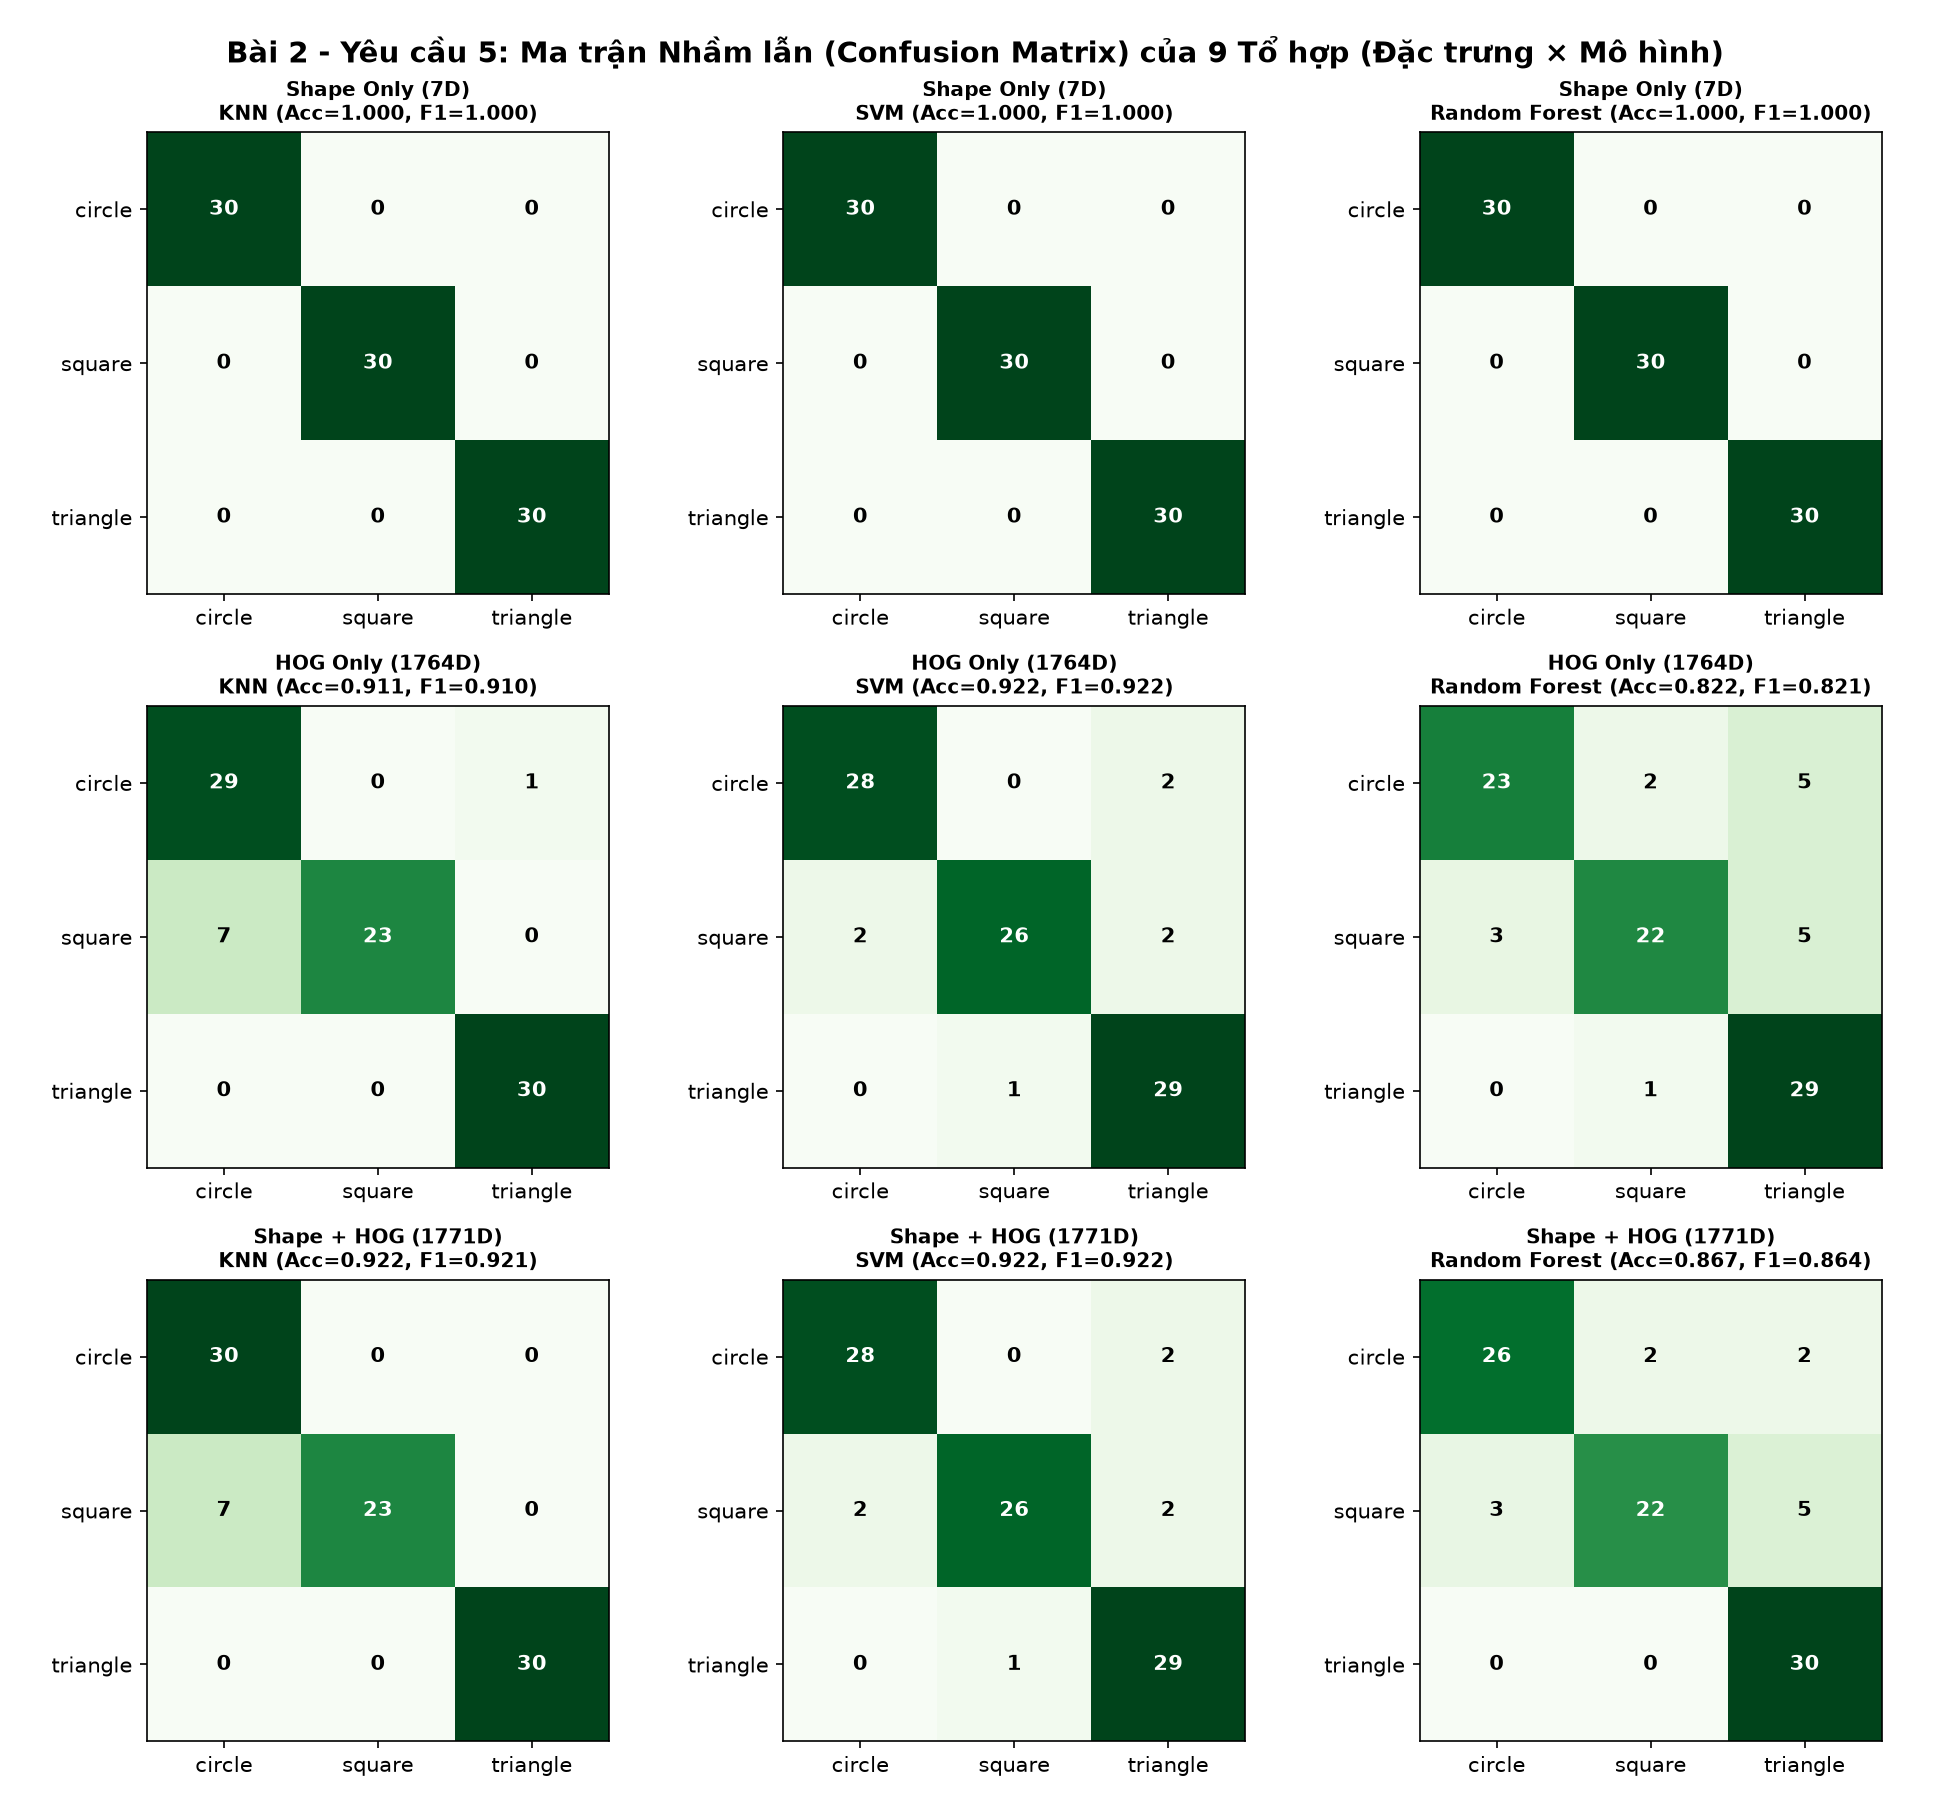
\includegraphics[width=0.92\textwidth]{outputs/bai2/fig4_confusion_matrices.png}
\caption{Ma trận nhầm lẫn (Confusion Matrix) của toàn bộ 9 tổ hợp (3 tập đặc trưng $\times$ 3 mô hình) trên tập Test.}
\label{fig:bai2_cm}
\end{figure}

\begin{figure}[H]
\centering
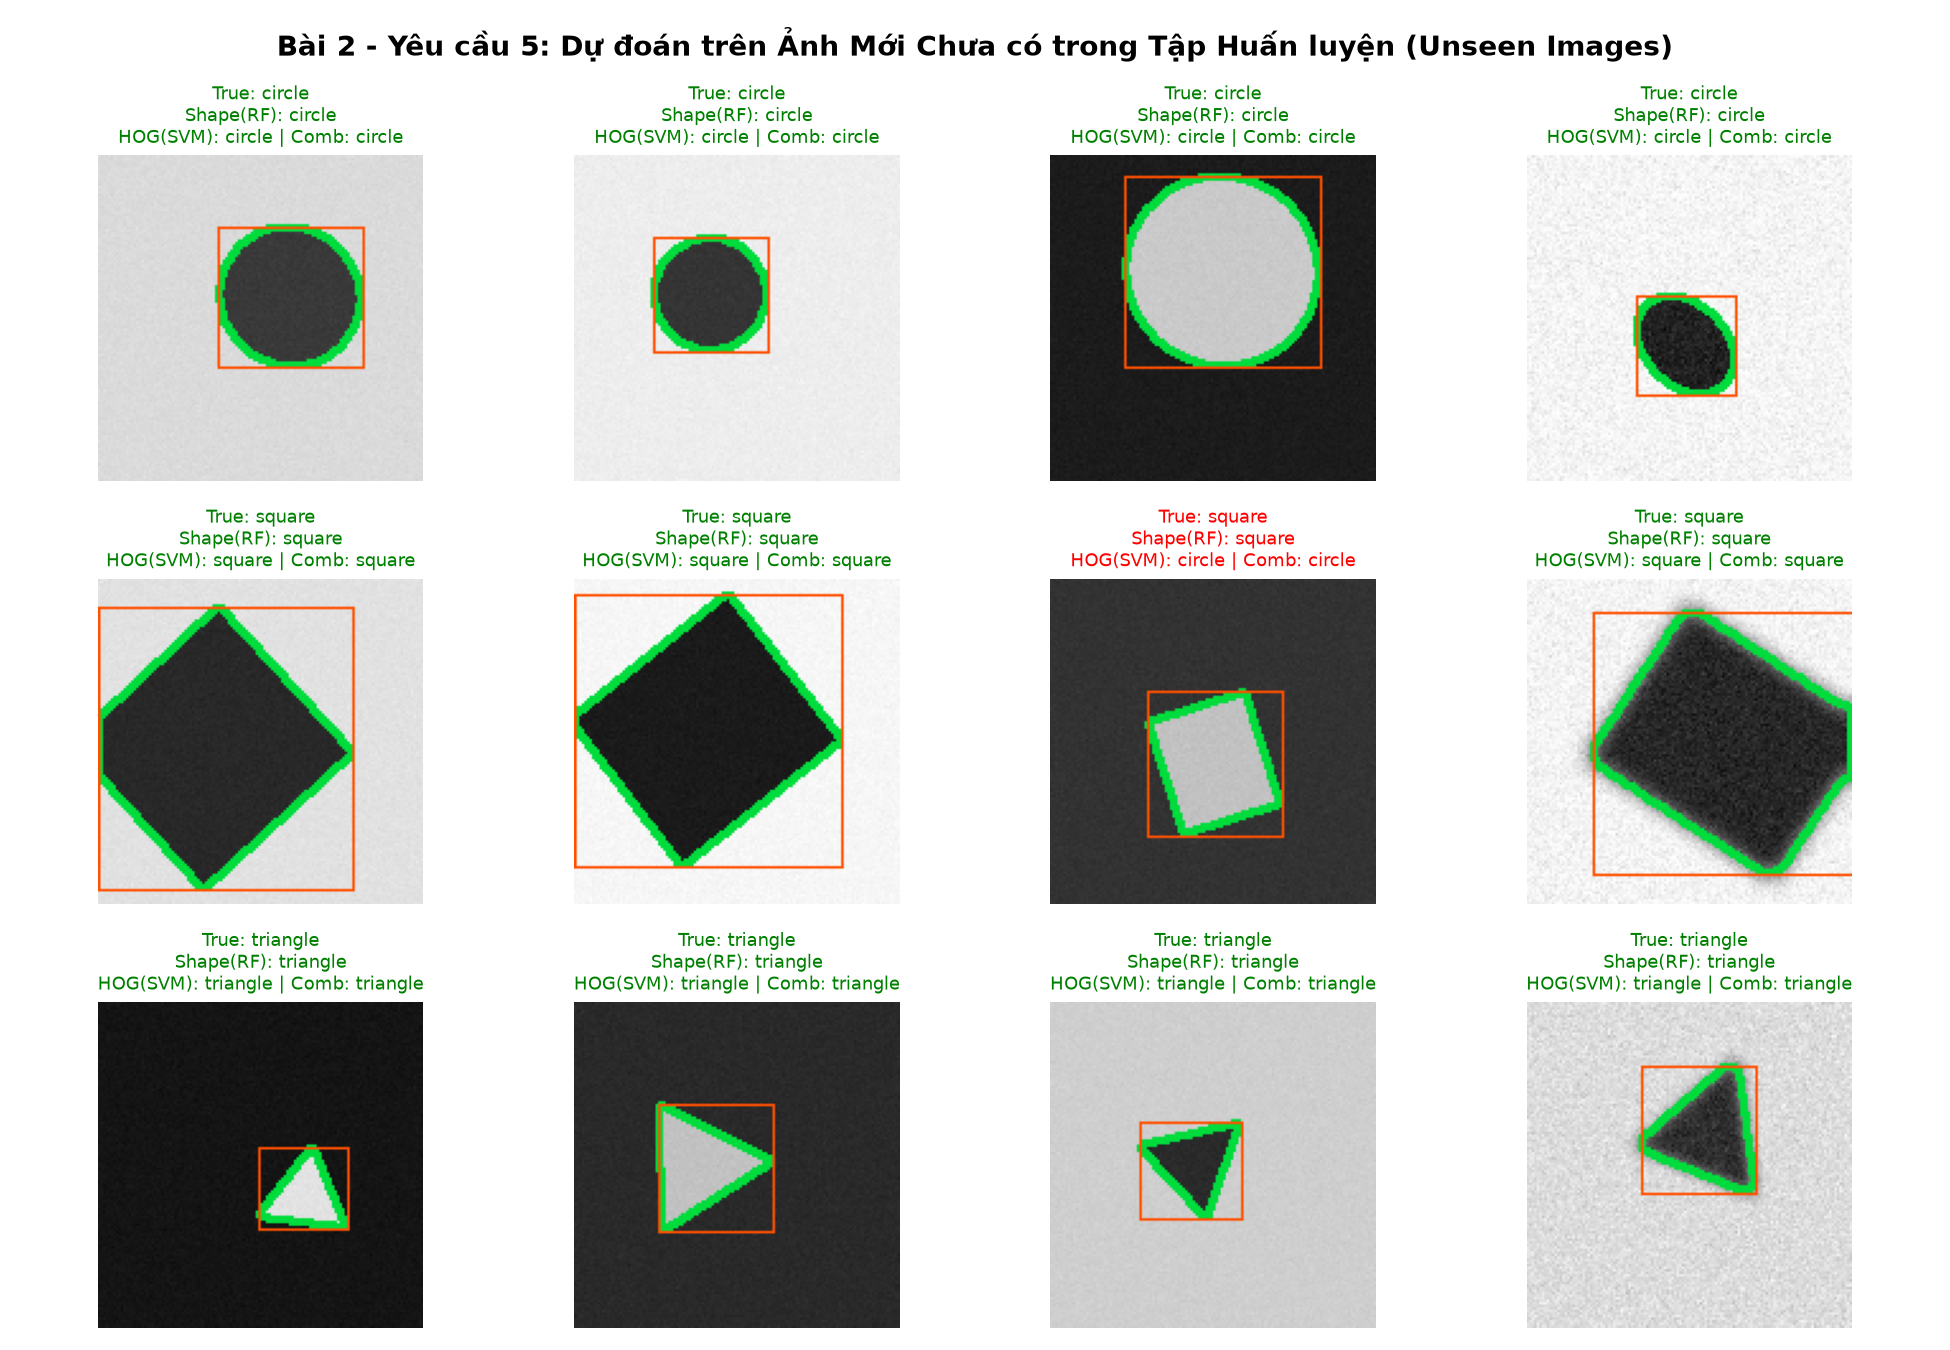
\includegraphics[width=0.95\textwidth]{outputs/bai2/fig5_unseen_predictions.png}
\caption{Kết quả dự đoán trên 12 ảnh mới chưa có trong tập huấn luyện (Unseen Images) ở Bài 2.}
\label{fig:bai2_unseen}
\end{figure}

\begin{figure}[H]
\centering
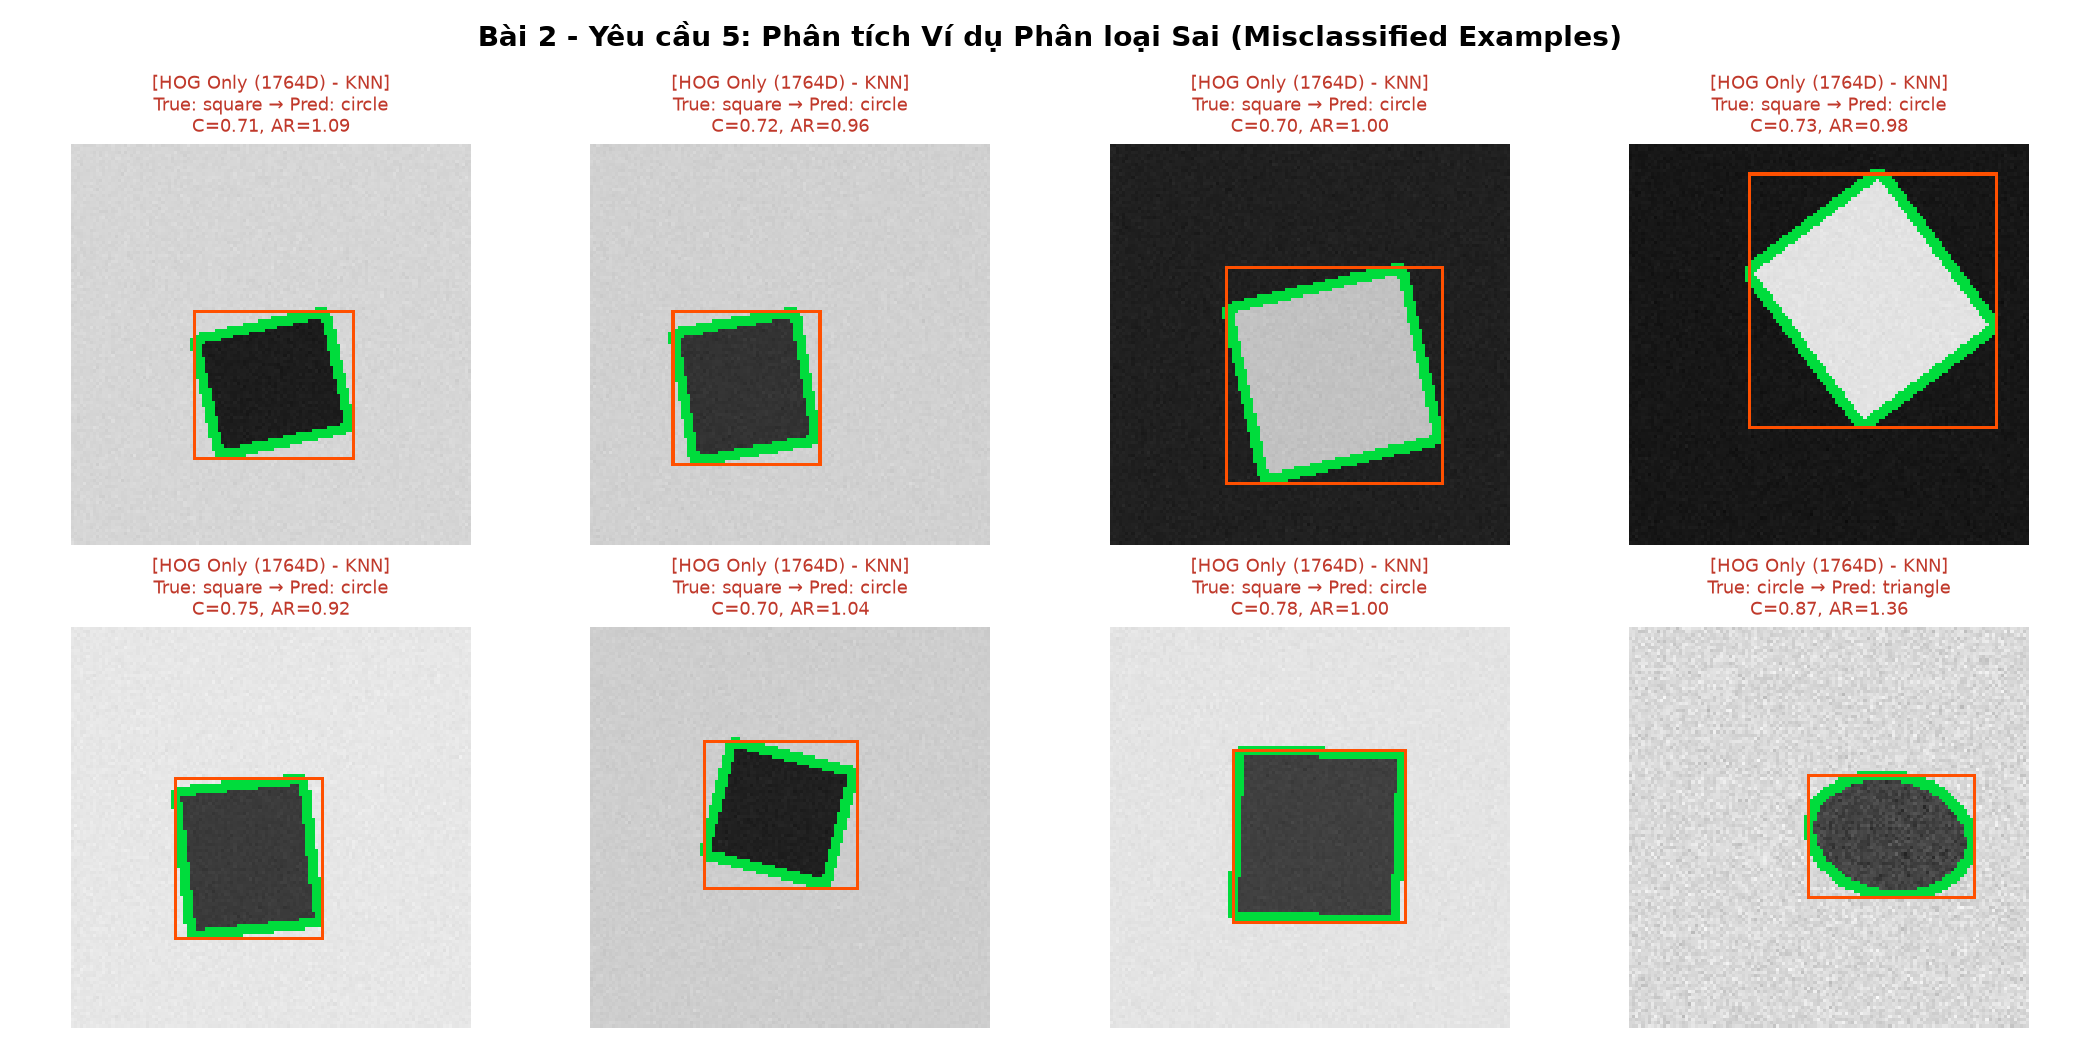
\includegraphics[width=0.96\textwidth]{outputs/bai2/fig6_misclassified_analysis.png}
\caption{Phân tích trực quan các ví dụ bị phân loại sai trên tập Test khi sử dụng đặc trưng HOG.}
\label{fig:bai2_mis}
\end{figure}

\subsubsection*{Phân tích kết quả và các ví dụ phân loại sai}
\begin{itemize}
    \item \textbf{So sánh số chiều vector HOG và vector hình dạng:} Vector đặc trưng hình dạng chỉ gồm \textbf{7 chiều} cô đọng, trong khi vector HOG trên ảnh $64 \times 64$ có tới \textbf{1.764 chiều} (lớn gấp \textbf{252 lần}).
    \item \textbf{Hiệu năng giữa 3 trường hợp đặc trưng:}
    \begin{enumerate}
        \item \textit{Trường hợp 1 (Chỉ đặc trưng hình dạng - 7D):} Cả 3 mô hình KNN, SVM và Random Forest đều đạt độ chính xác tuyệt đối \textbf{100\%} trên tập Test. Nguyên nhân là đặc trưng độ tròn $C = 4\pi A/P^2$ tạo ra 3 khoảng giá trị tách biệt hoàn toàn giữa Hình tròn ($C \approx 0.892$), Hình vuông ($C \approx 0.737$) và Tam giác ($C \approx 0.556$), đồng thời bất biến hoàn toàn với vị trí tâm và góc xoay.
        \item \textit{Trường hợp 2 (Chỉ đặc trưng HOG - 1764D):} SVM đạt kết quả cao nhất (Accuracy = \textbf{92.22\%}), tiếp theo là KNN (\textbf{91.11\%}) và thấp nhất là Random Forest (\textbf{82.22\%}). SVM vượt trội hơn Random Forest trên HOG vì SVM tìm siêu phẳng phân cách tối ưu đồng thời trên toàn bộ không gian 1.764 chiều liên tục, trong khi mỗi cây quyết định của Random Forest chỉ tách trục đơn lẻ trên một tập con ngẫu nhiên gồm $\sqrt{1764} \approx 42$ chiều tại mỗi nút.
        \item \textit{Trường hợp 3 (Kết hợp Hình dạng + HOG - 1771D):} Việc bổ sung 7 chiều hình dạng vào 1.764 chiều HOG giúp cải thiện rõ rệt độ chính xác của KNN (từ 91.11\% lên 92.22\%) và Random Forest (từ 82.22\% lên 86.67\%). Tuy nhiên, kết quả vẫn thấp hơn khi dùng riêng 7 chiều hình dạng vì khi chuẩn hóa Z-score đồng đều cho mọi cột, 1.764 chiều của HOG chiếm tới $99.6\%$ tổng phương sai khoảng cách, làm lu mờ đóng góp của 7 chiều hình dạng.
    \end{enumerate}
    \item \textbf{Phân tích cụ thể các ví dụ phân loại sai (Hình \ref{fig:bai2_mis}):}
    Quan sát các mẫu bị phân loại sai trên Hình \ref{fig:bai2_mis} (ví dụ: hình vuông xoay nghiêng hoặc bị làm mờ góc có $C = 0.70 \div 0.78$ bị mô hình \texttt{HOG Only - KNN} dự đoán nhầm thành \texttt{circle}; hoặc hình elip dẹt có $AR = 1.36$ ở góc phải dưới bị nhầm thành \texttt{triangle}) cho thấy: do các đối tượng trong ảnh không nằm cố định ở chính giữa mà dịch chuyển tâm ngẫu nhiên trong khoảng $[44, 84]$ và xoay góc bất kỳ $0^\circ \div 360^\circ$, các cạnh của hình vuông rơi vào các ô lưới cell $8 \times 8$ khác nhau và phân tán đều năng lượng đạo hàm vào nhiều bin góc, làm biểu đồ HOG cục bộ của hình vuông xoay nghiêng trông giống với sự phân bố đa hướng của đường tròn.
\end{itemize}

\subsection{Trả lời câu hỏi thảo luận Bài 2 (Câu 12, 13, 14, 15)}

\subsubsection*{Câu 12. Vì sao đặc trưng hình dạng phân biệt được tròn, vuông và tam giác?}
\begin{itemize}
    \item Ba hình học cơ bản có mối quan hệ toán học bất biến giữa diện tích $A$ và bình phương chu vi $P^2$ được lượng hóa trực tiếp qua \textbf{Độ tròn (Circularity)} $C = \frac{4\pi A}{P^2}$:
    \begin{itemize}
        \item \textbf{Hình tròn:} Không có góc nhọn, đạt diện tích tối đa cho một chu vi cho trước $\Rightarrow C_{\text{lý thuyết}} = 1.0$ (thực nghiệm trung bình đạt $0.892$).
        \item \textbf{Hình vuông:} Có 4 góc vuông, chu vi dài hơn đường tròn cùng diện tích $\Rightarrow C_{\text{lý thuyết}} = \frac{\pi}{4} \approx 0.785$ (thực nghiệm trung bình đạt $0.737$).
        \item \textbf{Hình tam giác:} Có 3 góc nhọn, tỷ lệ chu vi trên diện tích lớn nhất trong 3 hình $\Rightarrow C_{\text{lý thuyết}} = \frac{\pi}{3\sqrt{3}} \approx 0.604$ (thực nghiệm trung bình đạt $0.556$).
    \end{itemize}
    \item Kết hợp thêm diện tích $A$, chu vi $P$ và mật độ biên $ED$, các lớp đối tượng tạo thành 3 cụm tách rời hoàn toàn trong không gian 7 chiều, giúp mọi mô hình (KNN, SVM, Random Forest) dễ dàng phân loại chính xác 100\%.
\end{itemize}

\subsubsection*{Câu 13. HOG mô tả thông tin gì?}
\begin{itemize}
    \item \textbf{HOG (Histogram of Oriented Gradients)} mô tả \textbf{cấu trúc hình dáng cục bộ và diện mạo cạnh biên} của đối tượng thông qua sự phân bố (histogram) của \textbf{độ lớn và hướng đạo hàm mức xám (gradient orientation)} trong từng ô lưới không gian nhỏ (\textit{cells} $8 \times 8$ pixel).
    \item Cụ thể, tại mỗi ô con, HOG thống kê xem biên của vật thể đang nghiêng theo góc nào (chia thành 9 hướng từ $0^\circ \div 180^\circ$) và cường độ biên mạnh hay yếu, sau đó chuẩn hóa tương phản theo từng cụm ô (\textit{blocks} $16 \times 16$ pixel) để tăng khả năng chống chịu với sự thay đổi độ sáng và bóng đổ cục bộ.
\end{itemize}

\subsubsection*{Câu 14. Thay đổi kích thước hoặc góc quay ảnh hưởng ra sao?}
\begin{itemize}
    \item \textbf{Đối với đặc trưng hình dạng:}
    \begin{itemize}
        \item \textit{Thay đổi kích thước (Scale):} Làm thay đổi mạnh các đặc trưng tuyệt đối như Diện tích ($A$ tỉ lệ với $s^2$), Chu vi ($P$ tỉ lệ với $s$) và $W, H$. Tuy nhiên, các đặc trưng tỉ lệ không thứ nguyên như \textbf{Độ tròn ($C = 4\pi A/P^2$)} và \textbf{Tỷ lệ khung bao ($AR = W/H$)} hoàn toàn \textbf{bất biến với kích thước} (do hệ số tỉ lệ $s^2$ ở tử số và mẫu số tự triệt tiêu).
        \item \textit{Thay đổi góc quay (Rotation):} Diện tích $A$, Chu vi $P$ và Độ tròn $C$ hoàn toàn \textbf{bất biến với phép quay}. Riêng $W, H$ của khung bao đứng (\texttt{boundingRect}) sẽ dao động nhẹ khi hình vuông hoặc tam giác xoay nghiêng $45^\circ$.
    \end{itemize}
    \item \textbf{Đối với đặc trưng HOG:}
    \begin{itemize}
        \item \textit{Thay đổi kích thước và vị trí:} Nếu tính HOG trên toàn ảnh cố định mà không cắt (crop) theo khung bao đối tượng rồi chuẩn hóa về cùng kích thước, khi vật thể thu nhỏ/phóng to hoặc dịch chuyển tâm, các cạnh biên sẽ rơi vào các ô lưới (cell) khác nhau làm vector HOG thay đổi hoàn toàn.
        \item \textit{Thay đổi góc quay:} HOG \textbf{không bất biến với phép quay}. Khi đối tượng xoay một góc $\Delta\theta$, toàn bộ hướng gradient dịch chuyển sang các bin góc khác trong histogram 9 hướng, đồng thời vị trí không gian của các đỉnh/cạnh di chuyển sang các cell khác (đây chính là lý do ở Bài 2 khi góc quay biến thiên từ $0^\circ \div 360^\circ$, độ chính xác của HOG giảm xuống $82.2\% \div 92.2\%$).
    \end{itemize}
\end{itemize}

\subsubsection*{Câu 15. Khi nào nên dùng hình dạng, khi nào nên dùng HOG?}
\begin{itemize}
    \item \textbf{Nên dùng đặc trưng hình dạng (Contour Shape Descriptors) khi:}
    \begin{enumerate}
        \item Đối tượng có thể tách nền (segmentation/thresholding) rõ ràng để lấy được đường bao khép kín chính xác (như chi tiết cơ khí trên băng chuyền công nghiệp, biển báo giao thông hình học, tế bào trên kính hiển vi).
        \item Đối tượng trong ảnh có thể nằm ở vị trí bất kỳ, kích thước thay đổi hoặc xoay tự do $0^\circ \div 360^\circ$.
        \item Yêu cầu tốc độ tính toán thời gian thực cực nhanh trên thiết bị nhúng/robot với vector đặc trưng siêu gọn nhẹ (chỉ vài chiều số học).
    \end{enumerate}
    \item \textbf{Nên dùng đặc trưng HOG khi:}
    \begin{enumerate}
        \item Bối cảnh nền phức tạp, nhiễu hoặc độ tương phản không đồng đều khiến bước phân ngưỡng nhị phân (Otsu/Threshold) không thể tách rời được đường bao Contour chuẩn xác.
        \item Đối tượng có cấu trúc chi tiết bên trong phức tạp và hướng cố định (ví dụ: phát hiện người đi bộ đứng thẳng, nhận diện khuôn mặt, phương tiện giao thông, ký tự chữ viết đã căn chỉnh khung bao).
        \item Kết hợp với cửa sổ trượt đa tỉ lệ hoặc cắt vùng ROI chuẩn hóa kích thước kết hợp bộ phân loại tuyến tính/phi tuyến mạnh như SVM.
    \end{enumerate}
\end{itemize}

\end{document}
